% !TeX encoding = UTF8
% !TeX program = xelatex
\documentclass{cdut_thesis_twoside}
\usepackage{booktabs}
\usepackage{float}
\usepackage{subcaption}
\usepackage{bm}
\usepackage{multirow}
\usepackage{hologo}
\usepackage[super]{gbt7714}
\usepackage{pdfpages}
\usepackage{enumitem}
\usepackage{mhchem}
\usepackage{lscape}
\usepackage{metalogo}
\usepackage{enumitem}
\usepackage{colortbl}
\usepackage{framed}
\usepackage{rotfloat}
\usepackage{makecell}
\usepackage{diagbox} % 绘制表头斜线
\usepackage{listings}
    \renewcommand{\lstlistingname}{Code}
    \lstset{ %%用于列放python代码
        language=Python,
        basicstyle=\ttfamily\footnotesize,
        keywordstyle=\color{orange},
        stringstyle=\color{green},
        commentstyle=\color{red},
        frame=single,
        numbers=left,
        numberstyle=\tiny\color{gray},
        breaklines=true,
        showstringspaces=false,
        captionpos=t,
        escapeinside={(*@}{@*)} % 如果需要在代码中插入LaTeX命令,可以使用 (*@ ... @*) 包裹起来
    }

\definecolor{blueviolet}{RGB}{138, 43, 226}


\begin{document}

%----------------------------------------封面、摘要、目录----------------------------------------%
\thispagestyle{empty}
\begin{center}
    \makebox[109mm][c]{\heiti\zihao{-2} \cdut}              % \cdut 在类文件中定义为“成都理工大学普通本科实习报告”
\vskip2cm
    \makebox[109mm][c]{\heiti\zihao{2} \yourtitle}                     %报告的名称
\end{center}
\vskip2cm
\begin{center}
    \includegraphics[width=50mm,height=50mm]{school_badge/CDUT.png}                    %成都理工大学的校徽
\end{center}
\vskip2.5cm
%-------------------------------------------------个人信息---------------------------------------------------%
\begin{center}
    \makebox[30mm][l]{\heiti\zihao{3} 学 \hspace{0.8cm} 生:} \makebox[50mm][l]{\heiti\zihao{3} \yourname }
    %姓名
    \vskip0.5cm
    \makebox[30mm][l]{\heiti\zihao{3} 学 \hspace{0.8cm} 号:} \makebox[50mm][l]{\heiti\zihao{3} \yourstudentnumber }
    %学号
    \vskip0.5cm
    \makebox[30mm][l]{\heiti\zihao{3} 指导教师:} \makebox[50mm][l]{\heiti\zihao{3} \yourteacher }
    %指导教师
    \vskip0.5cm
    \makebox[30mm][l]{\heiti\zihao{3} 专 \hspace{0.8cm} 业:} \makebox[50mm][l]{\heiti\zihao{3} \yourmajor }
    %专业
\end{center}
%-------------------------------------------------个人信息---------------------------------------------------%
\vskip2.5cm
\begin{center}
    \makebox[109mm][c]{\heiti\zihao{-2} \yourcollege }    
\end{center}
\vskip1cm
\vfill\begin{center}
    {\heiti\zihao{3} \yourfinishdate }                                                   %撰写时间
\end{center}
\newpage
%-----------------------------空白页-----------------------------%
\makeatletter % 激活 @ 符号
\ifcdut@twoside % 文档为双面样式,则添加空白页
	\thispagestyle{empty}
	\null
	\newpage
\fi
\makeatother % 取消激活 @ 符号

%%%---------------------------------------(个人信息)要用时才做修改----------------------------------------%%%
%-----------------------------------------------------------------------------------------------------------%
%------------------------------------------------下划线格式--------------------------------------------------%
%\begin{center}
%    \makebox[30mm][l]{\heiti\zihao{3} 学 \hspace{0.8cm} 生:} \underline{\makebox[60mm][l]{\heiti\zihao{3} 安德利}}
%    %姓名
%    \vskip0.5cm
%    \makebox[30mm][l]{\heiti\zihao{3} 学 \hspace{0.8cm} 号:} \underline{\makebox[60mm][l]{\heiti\zihao{3} %202019020220}}
%    %学号
%    \vskip0.5cm
%    \makebox[30mm][l]{\heiti\zihao{3} 指导教师:} \underline{\makebox[60mm][l]{\heiti\zihao{3} 杜海英,吴灿,何鹏,徐婷婷}}
%    %指导教师
%    \vskip0.5cm
%    \makebox[30mm][l]{\heiti\zihao{3} 专 \hspace{0.8cm} 业:} \underline{\makebox[60mm][l]{\heiti\zihao{3} 环境科学与工程}}
%    %专业
%\end{center}
%------------------------------------------------下划线格式--------------------------------------------------%
%-----------------------------------------------------------------------------------------------------------%
%-------设置起始页脚------%
\setcounter{page}{1}
\pagenumbering{Roman}
%-------设置起始页脚------%
%--------------------摘要--------------------%
\null\par
\begin{chineseabstract}
    在本实验报告中,我学会了奥维互动地图(OMap)的使用,以及水、大气、土壤和声环境质量现状评价的实验方法和要求。首先,我学会了水环境质量评价中的标准指数法和内梅罗水质指数的应用。接着,我了解了大气环境质量评价中使用的AERSCREEN预测软件和EIAProA2018软件模型,以及制定大气环境监测方案的基本方法。然后,我熟悉了土壤环境质量调查的布点和采样分析方法,并根据最新的技术导则制定了土壤环境监测方案。最后,我掌握了声环境质量评价中使用的EIAN2.0和Surfer绘图软件软件进行影响预测的方法。

    通过这些实验,我掌握了不同环境领域的现状评价方法和工具的应用。我通过实践获得了评估水、大气、土壤和声环境质量的能力,并能够提出相应的改善建议。这些实验培养了我的环境保护意识,提高了解决环境问题的能力。

\par              %
\null             % 空
\par              % 两
\null             % 行
\par              %
\noindent \textbf{\heiti 关键词:} 水环境质量评价,大气环境质量评价,土壤环境质量调查,声环境质量评价,现状评价方法    %  (3-5个关键词)
\end{chineseabstract}


\null\par
\begin{englishabstract}
    In this experimental report, I learned the use of the Ovi Interactive Map (OMap) and the experimental methods and requirements for the evaluation of the current quality of water, atmosphere, soil and acoustic environment. First of all, I learned the standard index method and the application of Nemerow water quality index in water environment quality evaluation. Then, I learned about the AERSCREEN prediction software and EIAProA2018 software model used in the evaluation of atmospheric environmental quality, as well as the basic methods for developing atmospheric environmental monitoring programs. Then, I got familiar with the distribution and sampling analysis methods of soil environmental quality investigation, and formulated a soil environmental monitoring program according to the latest technical guidelines. Finally, I learned how to predict the impact of EIAN2.0 and Surfer mapping software software used in acoustic environment quality assessment.

    Through these experiments, I have mastered the application of current status assessment methods and tools in different environmental fields. Through practice, I have acquired the ability to evaluate the environmental quality of water, air, soil and sound, and can put forward corresponding suggestions for improvement. These experiments have cultivated my awareness of environmental protection and improved my ability to solve environmental problems.


\par              %
\null             % 空
\par              % 两
\null             % 行
\par              %
\noindent \textbf{Key words:} water environmental quality assessment, atmospheric environmental quality assessment, soil environmental quality investigation, sound environmental quality assessment, current status assessment methods    %  (3-5个关键词)
\end{englishabstract}
%--------------------摘要--------------------%
\null

{\thispagestyle{fancy}}                           % 设置目录的页眉页脚
\tableofcontents        %---------------生成目录
{\thispagestyle{fancy}}                           % 设置目录的页眉页脚

\newpage\null\par
\listoffigures        %---------------生成插图目录
{\thispagestyle{fancy}}                           % 设置目录的页眉页脚
\newpage\null\par
\listoftables         %---------------生成表格目录
{\thispagestyle{fancy}}                           % 设置目录的页眉页脚


\newpage
%----------------------------------------封面、摘要、目录----------------------------------------%
%----------------------------------------------正文----------------------------------------------%
%-------设置起始页脚------%
\setcounter{page}{1}
\pagenumbering{arabic}
%-------设置起始页脚------%
\null\par
\section{实验一\hspace{1em}水环境质量现状评价}
\subsection{教学目的与要求}

\noindent\textbf{教学目的:}通过几组水环境质量参数现状数据实例来进行水环境质量现状评价。
\newline\textbf{教学要求:}掌握标准指数法和内梅罗水质指数在水环境质量评价中的应用。


\subsection{实验报告背景}
\subsubsection[水质指数法]{水质指数法\protect\cite{HJ2.3-2018}}

\paragraph*{一般性水质因子(随着浓度增加而水质变差的水质因子)的指数计算公式:}
\begin{equation} \label{eq:General water quality factors}
    S_{i,j}=\dfrac{C_{i,j}}{C_{si}}
\end{equation}
式中:
$S_{i,j}$——评价因子 $i$ 的水质指数,大于1表明该水质因子超标;
\newline\phantom{式中:}$C_{i,j}$——评价因子 $i$ 在 $j$ 点的实测统计代表值,mg/L;
\newline\phantom{式中:}$C_{si}$——评价因子 $i$ 的水质评价标准限值,mg/L。

\paragraph*{溶解氧(DO)的标准指数计算公式:}
\begin{equation} \label{eq:DO}
    S_{\mathrm{DO},j} = 
    \begin{cases}
        \dfrac{\mathrm{DO_s}}{\mathrm{DO}_j} &\qquad \mathrm{DO}_j \leqslant \mathrm{DO_f} \\
        & \\
        \dfrac{\left\lvert \mathrm{DO_f}-\mathrm{DO}_j \right\rvert}{\mathrm{DO_f}-\mathrm{DO_s}} &\qquad \mathrm{DO}_j > \mathrm{DO_f}
    \end{cases}
\end{equation}
式中:
$S_{DO,j}$——溶解氧的标准指数,大于1表明该水质因子超标;
\newline\phantom{式中:}$\mathrm{DO}_j$——溶解氧在 $j$ 点的实测统计代表值,mg/L;
\newline\phantom{式中:}$\mathrm{DO_s}$——溶解氧的水质评价标准限值,mg/L;
\newline\phantom{式中:}$\mathrm{DO_f}$——饱和溶解氧浓度,mg/L,对于河流,$\mathrm{DO_f}=468/(31.6+T)$,对于
\newline\phantom{式中:$\mathrm{DO_f}$——}盐度比较高的湖泊、水库及入海河口、近岸海域,
\newline\phantom{式中:$\mathrm{DO_f}$——}$\mathrm{DO_f}=(491-2.65S)/(33.5+T)$;
\newline\phantom{式中:}$S$——实用盐度符号,量纲一;
\newline\phantom{式中:}$T$——水温,℃。

\paragraph*{pH值的指数计算公式:}
\begin{equation} \label{eq:pH}
    S_{\mathrm{pH},j} = 
    \begin{cases}
        \dfrac{7.0-\mathrm{pH}_j}{7.0-\mathrm{pH_{sd}}} &\qquad \mathrm{pH}_j \leqslant 7.0 \\
        & \\
        \dfrac{\mathrm{pH}_j-7.0}{\mathrm{pH_{su}}-7.0} &\qquad \mathrm{pH}_j > 7.0
    \end{cases}
\end{equation}
式中:
$S_{\mathrm{pH},j}$——pH值的指数,大于1表明该水质因子超标;
\newline\phantom{式中:}$\mathrm{pH}_j$——pH值实测统计代表值;
\newline\phantom{式中:}$\mathrm{pH_{sd}}$——评价标准中pH值的下限值;
\newline\phantom{式中:}$\mathrm{pH_{su}}$——评价标准中pH值的上限值。

\paragraph*{内梅罗水质指数计算公式:}
\begin{equation} \label{eq:Nemero Water Quality Index}
    P_{\text{传统}} = \sqrt{\dfrac{F_{\text{最大}}^2+F_{\text{平均}}^2}{2}}
\end{equation}
式中:
$P_{\text{传统}}$——传统内梅罗污染指数;
\newline\phantom{式中:}$F_{\text{最大}}$——$F_i$的最大值;
\newline\phantom{式中:}$F_{\text{平均}}$——$F_i$的平均值。


\subsubsection{计算标准要求}

\begin{enumerate}
    \item 使用单项指数法(标准指数法)和内梅罗水质指数评价某项目环评监测点的水质。
    \item 评价标准为《地表水环境质量标准》(GB3838-2002)中的Ⅲ类标准,各标准值见下表 \ref{tab:Environmental quality standards for surface water}。
\end{enumerate}

\begin{table}[H]
    \centering
    \caption{地表水环境质量标准\cite{GB3838-2002}}
    \resizebox{\textwidth}{!}{
    \begin{tabular}{ccccccccccc}
        \multicolumn{11}{r}{单位:mg/L,pH为无量纲,水温20℃} \\
        \toprule
        pH    & $\mathrm{COD_{Mn}}$ & $\mathrm{BOD_5}$  & DO    & SS    & 氨氮    & 总磷    & 总氮    & 石油类   & LAS   & 动植物油 \\
        \midrule
        $6\sim 9$   & $\leqslant 6$    & $\leqslant4$    & $\geqslant 5$    & $\leqslant100$  & $\leqslant1.0$  & $\leqslant0.05$ & $\leqslant1.0$  & $\leqslant0.05$ & $\leqslant0.2$  & $\leqslant0.05$ \\
        \bottomrule
    \end{tabular}}
    \label{tab:Environmental quality standards for surface water}%
\end{table}


\subsection{报告主体内容}
\subsubsection{水质情况}
\begin{table}[H]
    \centering
    \caption{某项目环评水质监测点结果}
    \begin{tabular}{cccccc}
        \multicolumn{6}{r}{单位:mg/L,pH为无量纲} \\
        \toprule
        序号    & 污染物   & 红路水库北 & 红路水库南 & 石场水坑  & 流溪河灌渠 \\
        \midrule
        1     & pH    & 7.7   & 7.97  & 7.9   & 7.5 \\
        2     & DO    & 7.0     & 6.8   & 7.3   & 6.1 \\
        3     & $\mathrm{BOD_5}$  & 2$^{\mathrm{L}}$    & 2$^{\mathrm{L}}$     & 2$^{\mathrm{L}}$    & 3.05 \\
        4     & $\mathrm{COD_{Mn}}$ & 5.3   & 5.3   & 1.8   & 3.23 \\
        5     & 氨氮    & 0.26  & 0.24  & 0.05  & 0.27 \\
        6     & SS    & 54.0    & 48.0    & 28.0    & 37.0 \\
        7     & 总磷    & 0.04  & 0.11  & 0.10   & 0.18 \\
        8     & 总氮    & 1.30   & 1.06  & 1.03  & 1.22 \\
        9     & 石油类   & 0.2   & 0.21  & 0.02$^{\mathrm{L}}$ & 0.02$^{\mathrm{L}}$ \\
        10    & LAS   & 0.14  & 0.13  & 0.05$^{\mathrm{L}}$ & 0.17 \\
        11    & 动植物油  & 0.37  & 0.35  & 0.02$^{\mathrm{L}}$ & 0.45 \\
        \bottomrule
        \multicolumn{6}{l}{备注:低于最低检测浓度,结果以最低检出浓度右上角加L表示。} \\
    \end{tabular}%
    \label{tab:Results of water quality monitoring points for environmental impact assessment of a project}%
\end{table}%


\subsubsection{Excel处理步骤}
\begin{enumerate}
    \item 数据整合
    \begin{enumerate}[label=(\arabic*)]
        \item 根据《地表水环境质量标准》(GB3838-2002)中的 Ⅲ 类标准(见表 \ref{tab:Environmental quality standards for surface water})和某项目环评水质监测点结果(见表 \ref{tab:Results of water quality monitoring points for environmental impact assessment of a project})将它们穿插排列:
        \begin{itemize}
            \item 上行为水质监测点结果,下行为地表水环境质量标准;
            \item 留出空位填写计算后相应的水质指数,并用横线将不同类别的污染物分开。
        \end{itemize}
        \item 再根据公式 \ref{eq:Nemero Water Quality Index} 的计算要求,在Excel末端插入三行空白栏位(分别为最大值、平均值和$P_{\text{传统}}$);
        \item 最后添加适当的分割线作为修饰,并绘制于 $\mathrm{A1:F26}$ 区域(版式效果可见表 \ref{tab:Evaluation of water quality parameters})。
    \end{enumerate}

    \item pH 值的指数计算
    \begin{enumerate}[label=(\arabic*)]
        \item 根据公式 \ref{eq:pH} 计算要求,获取到评价标准中:
        \begin{itemize}
            \item pH 值的下限值 $\mathrm{pH_{sd}}=6$
            \item pH 值的上限值 $\mathrm{pH_{su}}=9$
        \end{itemize}
        \item 然后通过IF函数对每个计算的值进行判断,以相对应的计算公式输出结果:
        \begin{align*}
            \mathrm{=IF(C\$2<=7,(7-C\$2)/(7-6),(C\$2-7)/(9-7))}
        \end{align*}
        \item 最后在pH栏位中依次向右自动填充。
    \end{enumerate}
    
    \item 溶解氧(DO)的标准指数计算
    \begin{enumerate}[label=(\arabic*)]
        \item 根据公式 \ref{eq:DO} 计算要求,又因为该项目环评处于河流段,且水温为20℃,则饱和溶解氧浓度为:
        $$\mathrm{DO_f}=468/(31.6+T)=468/(31.6+20) \;\text{mg/L}$$ 
        \item 通过IF函数对每个计算的值进行判断,以相对应的计算公式输出结果:
        \begin{align*}
            = & \mathrm{IF(C\$4<=(468/(31.6+20)),5/C\$4,} \\
            & \mathrm{ABS((468/(31.6+20))-C\$4)/((468/(31.6+20))-5))}
        \end{align*}
        \item 最后在DO栏位中依次向右自动填充。
    \end{enumerate}
    
    \item 一般性水质因子的指数计算
    
    相较于pH 值的指数计算和溶解氧(DO)的标准指数计算,一般性水质因子的指数计算就显得非常简单,根据公式 \ref{eq:General water quality factors} 计算要求,输入计算公式后自动填充即可。

    \item 创建Excel规则
    
    水质因子超标的要求是水质指数大于1,单单是自己一个一个比对的话,会非常吃力,但如果在Excel中建立相关规则就可以事半功倍。具体操作如下:
    \begin{enumerate}[label=(\arabic*)]
        \item 选中所有水质指数的计算单元格,点击“条件格式”中的“新建规则”;
        \item 选择“使用公式确定要设置格式的单元格”并在“为符合此公式的值设置格式”中输入“$\mathrm{=C2>1}$”(C2为所有选中单元格的首个单元格);
        \item 将格式样式设置为单元格背景填充为红色。
    \end{enumerate}
    通过以上操作即可完成规则的创建,也就得到了表 \ref{tab:Evaluation of water quality parameters} 展示的效果。

    \item 内梅罗水质指数$P_{\text{传统}}$的计算
    
    根据公式 \ref{eq:Nemero Water Quality Index} 要求,通过MAXIFS函数得到$F_{\text{最大}}$,AVERAGEIF函数得到$F_{\text{平均}}$,最后由计算公式得到 $P_{\text{传统}}$。以pH的操作举例:
    \begin{enumerate}[label=(\arabic*)]
        \item $F_{\text{最大}}$:$\mathrm{=MAXIFS(C\$1:C\$23,\$A\$1:\$A\$23,\text{"标准"})}$
        \item $F_{\text{平均}}$:$\mathrm{=AVERAGEIF(\$A\$1:\$A\$23,\text{"标准"},C\$1:C\$23)}$
        \item $P_{\text{传统}}$:$\mathrm{=((C\$24\text{\textasciicircum} 2+C\$25\text{\textasciicircum} 2)/2)\text{\textasciicircum} 0.5}$
        \item 最后全部依次向右自动填充。
    \end{enumerate}
\end{enumerate}

经过以上Excel的处理步骤,可以得到完整的水质参数评价结果,如下表 \ref{tab:Evaluation of water quality parameters} 所示。


\subsubsection{水质参数评价结果与分析}
% \begin{table}[H]
%     \centering
%     \caption{水质参数评价结果}
%     \resizebox{\textwidth}{!}{
%     \begin{tabular}{cc|cccc|cc|c}
%         \specialrule{1pt}{0pt}{0pt} % 1pt是线宽
%         序号    & 污染物   & 红路水库北 & 红路水库南 & 石场水坑  & 流溪河灌渠 & 最大值   & 平均值   & $P_{\text{传统}}$ \\
%         \hline
%         1     & pH    & 7.70  & 7.97  & 7.90  & 7.5   &       &       &  \\
%         标准    & $6\sim 9$   & 0.350  & 0.485  & 0.450  & 0.250  & 0.485  & 0.3838  & 0.4373  \\
%         \hline
%         2     & DO    & 7.0   & 6.8   & 7.3   & 6.1   &       &       &  \\
%         标准    & $\geqslant 5$    & 0.714  & 0.735  & 0.685  & 0.820  & 0.820  & 0.7385  & 0.7802  \\
%         \hline
%         3     & BOD$_5$  & 2     & 2     & 2     & 3.05  &       &       &  \\
%         标准    & $\leqslant 4$    & 0.500  & 0.500  & 0.500  & 0.763  & 0.763  & 0.5656  & 0.6713  \\
%         \hline
%         4     & $\mathrm{COD_{Mn}}$ & 5.3   & 5.3   & 1.8   & 3.23  &       &       &  \\
%         标准    & $\leqslant 6$    & 0.883  & 0.883  & 0.300  & 0.538  & 0.883  & 0.6513  & 0.7760  \\
%         \hline
%         5     & 氨氮    & 0.26  & 0.24  & 0.05  & 0.27  &       &       &  \\
%         标准    & $\leqslant 1.0$  & 0.260  & 0.240  & 0.050  & 0.270  & 0.270  & 0.2050  & 0.2397  \\
%         \hline
%         6     & SS    & 54.0  & 48.0  & 28.0  & 37.0  &       &       &  \\
%         标准    & $\leqslant 100$  & 0.540  & 0.480  & 0.280  & 0.370  & 0.540  & 0.4175  & 0.4827  \\
%         \hline
%         7     & 总磷    & 0.04  & 0.11  & 0.10  & 0.18  &       &       &  \\
%         标准    & $\leqslant 0.05$ & 0.800  & \cellcolor[rgb]{ 1,  0,  0}2.200  & \cellcolor[rgb]{ 1,  0,  0}2.000  & \cellcolor[rgb]{ 1,  0,  0}3.600  & 3.600  & 2.1500  & \cellcolor[rgb]{ 1,  0,  0}2.9650  \\
%         \hline
%         8     & 总氮    & 1.30  & 1.06  & 1.03  & 1.22  &       &       &  \\
%         标准    & $\leqslant 1.0$  & \cellcolor[rgb]{ 1,  0,  0}1.300  & \cellcolor[rgb]{ 1,  0,  0}1.060  & \cellcolor[rgb]{ 1,  0,  0}1.030  & \cellcolor[rgb]{ 1,  0,  0}1.220  & 1.300  & 1.1525  & \cellcolor[rgb]{ 1,  0,  0}1.2285  \\
%         \hline
%         9     & 石油类   & 0.20  & 0.21  & 0.02  & 0.02  &       &       &  \\
%         标准    & $\leqslant 0.05$ & \cellcolor[rgb]{ 1,  0,  0}4.000  & \cellcolor[rgb]{ 1,  0,  0}4.200  & 0.400  & 0.400  & 4.200  & 2.2500  & \cellcolor[rgb]{ 1,  0,  0}3.3692  \\
%         \hline
%         10    & LAS   & 0.14  & 0.13  & 0.05  & 0.17  &       &       &  \\
%         标准    & $\leqslant 0.2$  & 0.700  & 0.650  & 0.250  & 0.850  & 0.850  & 0.6125  & 0.7408  \\
%         \hline
%         11    & 动植物油  & 0.37  & 0.35  & 0.02  & 0.45  &       &       &  \\
%         标准    & $\leqslant 0.05$ & \cellcolor[rgb]{ 1,  0,  0}7.400  & \cellcolor[rgb]{ 1,  0,  0}7.000  & 0.400  & \cellcolor[rgb]{ 1,  0,  0}9.000  & 9.000  & 5.9500  & \cellcolor[rgb]{ 1,  0,  0}7.6290  \\
%         \specialrule{1pt}{0pt}{0pt} % 1pt是线宽
%     \end{tabular}}
%     \label{tab:Evaluation of water quality parameters}%
% \end{table}%

\begin{table}[H]
    \centering
    \caption{水质参数评价结果}
    \begin{tabular}{cc|cccc}
        \specialrule{1pt}{0pt}{0pt} % 1pt是线宽
        序号 & 污染物 & 红路水库北 & 红路水库南 & 石场水坑 & 流溪河灌渠 \\
        \hline
        1 & pH & 7.70 & 7.97 & 7.90 & 7.5 \\
        标准 & $6\sim 9$ & 0.350 & 0.485 & 0.450 & 0.250 \\
        \hline
        2 & DO & 7.0 & 6.8 & 7.3 & 6.1 \\
        标准 & $\geqslant 5$ & 0.714 & 0.735 & 0.685 & 0.820 \\
        \hline
        3 & BOD$5$ & 2 & 2 & 2 & 3.05 \\
        标准 & $\leqslant 4$ & 0.500 & 0.500 & 0.500 & 0.763 \\
        \hline
        4 & $\mathrm{COD{Mn}}$ & 5.3 & 5.3 & 1.8 & 3.23 \\
        标准 & $\leqslant 6$ & 0.883 & 0.883 & 0.300 & 0.538 \\
        \hline
        5 & 氨氮 & 0.26 & 0.24 & 0.05 & 0.27 \\
        标准 & $\leqslant 1.0$ & 0.260 & 0.240 & 0.050 & 0.270 \\
        \hline
        6 & SS & 54.0 & 48.0 & 28.0 & 37.0 \\
        标准 & $\leqslant 100$ & 0.540 & 0.480 & 0.280 & 0.370 \\
        \hline
        7 & 总磷 & 0.04 & 0.11 & 0.10 & 0.18 \\
        标准 & $\leqslant 0.05$ & 0.800 & \cellcolor[rgb]{ 1, 0, 0}2.200 & \cellcolor[rgb]{ 1, 0, 0}2.000 & \cellcolor[rgb]{ 1, 0, 0}3.600 \\
        \hline
        8 & 总氮 & 1.30 & 1.06 & 1.03 & 1.22 \\
        标准 & $\leqslant 1.0$ & \cellcolor[rgb]{ 1, 0, 0}1.300 & \cellcolor[rgb]{ 1, 0, 0}1.060 & \cellcolor[rgb]{ 1, 0, 0}1.030 & \cellcolor[rgb]{ 1, 0, 0}1.220 \\
        \hline
        9 & 石油类 & 0.20 & 0.21 & 0.02 & 0.02 \\
        标准 & $\leqslant 0.05$ & \cellcolor[rgb]{ 1, 0, 0}4.000 & \cellcolor[rgb]{ 1, 0, 0}4.200 & 0.400 & 0.400 \\
        \hline
        10 & LAS & 0.14 & 0.13 & 0.05 & 0.17 \\
        标准 & $\leqslant 0.2$ & 0.700 & 0.650 & 0.250 & 0.850 \\
        \hline
        11 & 动植物油 & 0.37 & 0.35 & 0.02 & 0.45 \\
        标准 & $\leqslant 0.05$ & \cellcolor[rgb]{ 1, 0, 0}7.400 & \cellcolor[rgb]{ 1, 0, 0}7.000 & 0.400 & \cellcolor[rgb]{ 1, 0, 0}9.000 \\
        \hline
        \multicolumn{2}{c|}{最大值} & 7.400  & 7.000  & 2.000  & 9.000  \\
        \multicolumn{2}{c|}{平均值} & 1.5861  & 1.6758  & 0.5768  & 1.6437  \\
        \hline
        \multicolumn{2}{c|}{P传统} & 5.3514  & 5.0896  & 1.4719  & 6.4692  \\
        \specialrule{1pt}{0pt}{0pt} % 1pt是线宽
    \end{tabular}
    \label{tab:Evaluation of water quality parameters}%
\end{table}


根据表格中的计算数据,可以得到以下信息:
\begin{enumerate}
    \item pH值、溶解氧(DO)、五日生化需氧量(BOD$_5$)、高锰酸盐指数($\mathrm{COD_{Mn}}$)、氨氮、悬浮物(SS)和线性烷基苯磺酸盐(LAS)的浓度均满足标准要求。
    \item 红路水库南和红路水库北的总磷和总氮超过了标准值,表明水库的富营养化程度较高,需要采取相应的措施进行治理。
    \item 石场水坑、流溪河灌渠、红路水库北的石油类和动植物油超过了标准值,说明这些地点存在油类污染物的排放,需要加强监管和减少排放。
    \item 内梅罗水质指数值$P_{\text{传统}}$越大,表示水质状况越差;反之,如果内梅罗水质指数值$P_{\text{传统}}$较小,表示水质状况较好。从计算出的 $P_{\text{传统}}$ 可以看出,除了石场水坑,红路水库北、红路水库南和流溪河灌渠的$P_{\text{传统}}$都比较大,水质污染情况较为严重,需要关注和加强相关处理,减少其主要污染物的排放或产生。
\end{enumerate}

在水质污染评价中,我们还可以根据内梅罗水质指数污染程度的不同来划分等级标准,以判断水质的污染程度,并进行相应的评价和管理:
\begin{table}[H]
    \centering
    \caption{内梅罗水质指数污染等级划分标准}
    \begin{tabular}{cccccc}
    \toprule
    P     & <1    & $1\sim 2$   & $2\sim 3$   & $3\sim 5$   & >5 \\
    \midrule
    水质等级  & 清洁    & 轻污染   & 污染    & 重污染   & 严重污染 \\
    \bottomrule
    \end{tabular}
    \label{tab:Nemero Water Quality Index pollution classification standard}
\end{table}

根据内梅罗水质指数污染等级划分标准,我们可以进一步将区域污染程度进行可视化的等级评价:
\begin{table}[H]
    \centering
    \caption{区域污染等级评价}
      \begin{tabular}{ccc}
      \toprule
      区域    & $P_{\text{传统}}$   & 水质等级 \\
      \midrule
      红路水库北 & 5.3514  & 严重污染 \\
      红路水库南 & 5.0896  & 严重污染 \\
      石场水坑  & 1.4719  & 轻污染 \\
      流溪河灌渠 & 6.4692  & 严重污染 \\
      \bottomrule
      \end{tabular}%
    \label{tab:Regional pollution level evaluation}%
\end{table}%



\subsection{小结及建议}

在采取措施改善水质的时候,需要关注水质因子指数较高的监测点,特别是对红路水库南、红路水库北和流溪河灌渠的治理更为紧迫。以下是一些建议和意见:
\begin{enumerate}
    \item 总磷和总氮的超标可能与农业、污水排放等因素有关。建议加强农田和养殖场的管理,合理使用化肥和农药,并加强污水处理,以降低排放对水体的影响。
    \item 石油类和动植物油的超标可能与工业废水排放、油污等因素有关。建议严格控制工业废水的排放,加强油污治理和监管,确保工业和生活污水得到有效处理,避免对水体造成污染。
    \item 需要建立有效的监测和预警机制,及时发现和应对水质问题。定期对水质进行监测,并进行综合评估和分析,以便及时采取措施进行治理和改善。
    \item 提高公众的环保意识,加强环境教育,鼓励居民、企业和机构积极参与水质保护和治理工作,共同建设美丽的水环境。
\end{enumerate}

水质问题是一个复杂的系统工程,需要多方合作和持续努力才能取得明显的改善效果。希望相关部门和社会各界共同努力,保护和改善水环境,为人民群众提供更好的生活条件。

 % 实验一部分 水
\newpage\null\par
\section{实验二\hspace{1em}大气环境质量现状评价}
\subsection{教学目的与要求}
\noindent\textbf{教学目的:}通过某城市生活垃圾环保发电厂为实例来进行大气环境质量评价。\newline
\noindent\textbf{教学要求:}
\begin{enumerate}
    \item 熟悉大气环境预测软件AERSCREEN在大气环境质量预测与评价中的应用,掌握EIAProA2018软件模型估算最大落地浓度和$\mathrm{D_{10\%}}$确定评价工作等级的基本方法。
    \item 利用EIAProA2018软件估算最大落地浓度和$\mathrm{D_{10\%}}$确定评价工作等级和范围,并附上软件主要操作步骤。
    \item 制定某城市生活垃圾环保发电厂的大气环境质量现状监测方案(包含范围、布点(按要求给出布点图)、因子、方法、时期、次数等)。
\end{enumerate}

\subsection{实验报告背景}
\begin{enumerate}
    \item 确定某城市生活垃圾环保发电厂大气环境质量评价工作等级与评价范围
    
    根据项目初步分析,选择 $1\sim3$ 种主要污染物,分别计算每一种污染物的最大地面浓度占标率 $P_i$(第 $i$ 个污染物),及第 $i$ 个污染物的地面浓度达标准限值10\%时所对应的最远距离$\mathrm{D_{10\%}}$。
    \begin{equation} \label{eq:The maximum ground concentration of the pollutant is standardized}
        P_i=\dfrac{C_i}{C_{0i}}\times 100\%
    \end{equation}
    式中:$P_i$——第i个污染物的最大地面空气质量浓度占标率,\%;
    \newline\phantom{式中:}$C_i$——采用估算模型计算出的第$i$个污染物的最大1 h地面空气质量浓度,μg/m$^3$;
    \newline\phantom{式中:}$C_{oi}$——第$i$个污染物的环境空气质量浓度标准,μg/m$^3$。一般选用GB 3095中1h平均质量浓度的二级浓度限值,如项目位于一类环境空气功能区,应选择相应的一级浓度限值;对该标准中未包含的污染物,使用评价标准\cite{HJ2.2-2018}确定的各评价因子1 h平均质量浓度限值。对仅有8h平均质量浓度限值、日平均质量浓度限值或年平均质量浓度限值的,可分别按2倍、3倍、6倍折算为1 h平均质量浓度限值。

    \begin{table}[H]
        \centering
        \caption{评价等级判别表\cite{HJ2.2-2018}}
        \begin{tabular}{cc}
        \toprule
        评价工作等级 & 评价工作分级判据 \\
        \midrule
        一级评价 & $P_{\text{max}} \geqslant  10\%$ \\
        二级评价 & $1\% \leqslant  P_{\text{max}} < 10\%$ \\
        三级评价 & $P_{\text{max}} < 1\%$ \\
        \bottomrule
        \end{tabular}
    \end{table}

    \item 污染源及项目周边条件基本信息
    
    \begin{table}[H]
        \centering
        \caption{污染源及项目周边条件基本信息}
        \begin{tabular}{p{0.3\textwidth}p{0.15\textwidth}p{0.1\textwidth}}
            \toprule
            名称 & 值 & 单位 \\
            \midrule
            污染源总量排放速率 & 60000 & Nm$^3$/h \\
            烟囱高度 & 130 & m \\
            烟囱内径 & 5 & m \\
            排放口温度 & 293 & K \\
            烟气出口速度 & 15 & m/s \\
            所在区域最低气温 & $-6$ & ℃ \\
            所在区域最高气温 & 44 & ℃ \\
            \midrule
            地点 & 农村地区 & - \\
            区域湿度条件 & 潮湿 & - \\
            \bottomrule
        \end{tabular}
        \label{tab:Basic information on pollution sources and surrounding conditions of the project}
    \end{table}

    \item 污染物标准
    
    计算污染物的源强(烟气流量与污染物浓度相乘),利用EIAProA2018软件估算出每个污染物的最大出落地浓度,再与环境空气质量标准(二级小时浓度)相比计算$P_i$。
    \begin{table}[H]
        \centering
        \caption{污染物排放值}
        \resizebox{\textwidth}{!}{
        \begin{tabular}{cccccc}
        \toprule
        序号    & 污染物名称 & 单位    & 工业企业设计卫生标准 & 项目排放值 & 污染源强(kg/h) \\
        \midrule
        1     & 颗粒物   & μg/Nm$^3$ & 900   & 50    & 0.003 \\
        2     & HCl   & μg/Nm$^3$ & 50    & 50    & 0.003 \\
        3     & HF    & μg/Nm$^3$ & 20    & 2     & 0.00012 \\
        4     & $\mathrm{SO_x}$   & μg/Nm$^3$ & 500   & 250   & 0.015 \\
        5     & $\mathrm{NO_x}$   & μg/Nm$^3$ & 250   & 150   & 0.009 \\
        6     & CO    & μg/Nm$^3$ & 10000 & 100   & 0.006 \\
        \bottomrule
        \end{tabular}}
        \label{tab:Pollutant emission value}%
    \end{table}%

    \item 制定某城市生活垃圾环保发电厂(成都九江环保发电有限公司)大气环境质量监测计划
    \begin{enumerate}[label=(\arabic*)]
        \item 监测范围
        \item 监测布点(图上标识,表格说明监测点基本信息)
        \item 监测因子
        \item 监测方法
        \item 监测时期
        \item 监测次数
    \end{enumerate}

    \item 奥维地图或谷歌地图或百度地图获取项目位置关系图
\end{enumerate}


\subsection{报告主体内容}
\subsubsection{标准浓度限值}
因为城市生活垃圾环保发电厂(成都九江环保发电有限公司)属于居住区、商业交通居民混合区、文化区、工业区和农村地区范围,归为第二类环境空气功能区,所以在遵守环境空气功能区质量要求时,使用二级浓度限值。\cite{GB3095-2012}

查阅《环境影响评价技术导则——大气环境》(HJ 2.2-2018)和《环境空气质量标准》(GB 3095-2012),并根据污染物的最大地面浓度占标率$P_i$的计算需求(见公式 \ref{eq:The maximum ground concentration of the pollutant is standardized}),得到项目排放污染物平均质量浓度的二级浓度限值,并汇总如下:

\begin{table}[H]
    \centering
    \caption{环境空气污染物浓度限值}
    \begin{tabular}{cccccc}
        \toprule
        污染物名称 & 1h平均  & 24h平均 & 年平均   & 单位    & 标准来源 \\
        \midrule
        PM2.5 & 217.5\footnotemark & 75   & 35    & μg/m$^3$ & GB 3095-2012 \\
        HCl   & 50    &  15   &       & μg/m$^3$ & HJ 2.2-2018 \\
        氟化物   & 20    & 7     &       & μg/m$^3$ & GB 3095-2012 \\
        SO2   & 500   & 150   & 60    & μg/m$^3$ & GB 3095-2012 \\
        NOx   & 250   & 100   & 25    & μg/m$^3$ & GB 3095-2012 \\
        CO    & 10    & 4     &       & mg/m$^3$ & GB 3095-2012 \\
        \bottomrule
    \end{tabular}
    \label{tab:Ambient air pollutant concentration limits}
\end{table}
\footnotetext{《环境影响评价技术导则——大气环境》(HJ 2.2-2018):对仅有8 h平均质量浓度限值、日平均质量浓度限值或年平均质量浓度限值的,可分别按2倍、3倍、6倍折算为1h平均质量浓度限值。所以,这里1h平均折算的方法为:$1\mathrm{h}\text{平均}=(24\mathrm{h}\text{平均}\times 3+\text{年平均}\times 6)/2$。}



\subsubsection{AERSCREEN估算模型}

\begin{framed}
\fangsong\footnotesize
\noindent 打开“../EIAPROA2018/AERMOD/AERSCREEN.exe”文件,并根据上表 \ref{tab:Basic information on pollution sources and surrounding conditions of the project} 提供的污染源及项目周边条件基本信息,开始估算:
\begin{itemize}[label=\textcolor{orange}{Prompt:}, align=left, leftmargin=*, itemsep=-0.5em]
    \item Enter Title:
    \item[Input:] Test1
    \item English or Metric Units? (E or M):
    \item[Input:] M
    \item POINT, VOLUME, AREA, AREACIRC, FLARE, POINTCAP, or POINTHO Source? (P, V, A, C, F, S, or H):
    \item[Input:] P
    \item Enter Emission Rate (g/s):
    \item[Input:] 21.548333 \\
    标准条件下空气的密度约为 1.2929 kg/m$^3$,所以 $60000 \;\mathrm{Nm^3/h} = (60000\times 1.2929)/3600 \;\mathrm{g/s} = 21.548333 \;\mathrm{g/s}$
    \item Enter Stack Height (meters):
    \item[Input:] 130
    \item Enter Stack Diameter (meters):
    \item[Input:] 5
    \item Enter Stack Temperature (K) \\
    Enter 0 for ambient temperature or a negative number for temperature
    difference ((K)) between stack temperature and ambient temperature:
    \item[Input:] -19.85 \\
    因为排放口温度为 293 K,则 $273.15-293 \;\text{K}=-19.85$ K
    \item Enter Option for Flow Rate or Exit Velocity: \\
    Option(1) - Exit Velocity (m/s) \\
    Option(2) - Exit Velocity (ft/s) \\
    Option(3) - Flow Rate (ACFM)
    \item[Input:] 1
    \item Enter Exit Velocity (m/s):
    \item[Input:] 15
    \item Rural or Urban? (R or U):
    \item[Input:] R
    \item Enter Minimum Distance (meters) to Ambient Air \\
    <Enter> for default (1 m):
    \item[Input:] 10 \\
    《环境影响评价技术导则——大气环境》(HJ 2.2-2018):估算模型AERSCREEN在距污染源10 m至25 km处默认为自动设置计算点,最远计算距离不超过污染源下风向50km。
    \item Enter an option for modeling NO2 chemistry: \\
    1) No chemistry or pollutant is not NO2 \\
    2) Use Ozone Limiting Method (OLM) \\
    3) Use Plume Volume Molar Ratio Method (PVMRM)
    \item[Input:] 1
    \item Include Building Downwash? (y/n):
    \item[Input:] n
    \item Include Terrain Heights? (y/n):
    \item[Input:] n
    \item Enter Maximum Distance (m) to probe \\
    <Enter> for default (5000 m):
    \item[Input:] 25000 \\
    《环境影响评价技术导则——大气环境》(HJ 2.2-2018):估算模型AERSCREEN在距污染源10 m至25 km处默认为自动设置计算点,最远计算距离不超过污染源下风向50km。
    \item Include up to 10 discrete receptors? (y/n):
    \item[Input:] n
    \item Use Flagpole receptors? (y or n):
    \item[Input:] n
    \item Enter source elevation (m) or <Enter> for default 0 m:
    \item[Input:] 0
    \item Enter Min \& Max Ambient Temperatures (K) or <Enter> to default to 250 310 K... \\
    Enter Minimum Temperature (K): \\
    Enter Maximum Temperature (K):
    \item[Input:] 267.15 \quad and \quad 317.15 \\
    $\text{Minimum Temperature} = -6+273.15 \;\text{K} = 267.15$ K \\
    $\text{Maximum Temperature} = 44+273.15 \;\text{K} = 317.15$ K
    \item Enter Minimum Wind Speed or <Enter> to default to 0.5 m/s...
    \item[Input:] 0.5 \\
    《环境影响评价技术导则——大气环境》(HJ 2.2-2018):估算模型AERSCREEN最小风速可取0.5 m/s。
    \item Enter Anemometer Height or <Enter> to default to 10.0 meters...
    \item[Input:] 10 \\
    《环境影响评价技术导则——大气环境》(HJ 2.2-2018):估算模型AERSCREEN风速计高度取10 m。
    \item Enter surface characteristics option: \\
    1) Single user specified values \\
    2) AERMET seasonal tables \\
    3) External file
    \item[Input:] 2
    \item Enter Dominant Surface Profile: \\
    1) Water \\
    2) Deciduous Forest \\
    3) Coniferous Forest \\
    4) Swamp \\
    5) Cultivated Land \\
    6) Grassland \\
    7) Urban \\
    8) Desert Shrubland
    \item[Input:] 7
    \item Enter Dominant Climate Profile: \\
    1) Average Moisture \\
    2) Wet Conditions \\
    3) Dry Conditions
    \item[Input:] 2
    \item Enter Y or y to adjust u* or N or n to not adjust u*
    \item[Input:] n
    \item Apply inversion break-up fumigation (y/n):
    \item[Input:] n
    \item Apply shoreline fumigation (y/n):
    \item[Input:] n
    \item Enter Y or y to turn on the debug option or <Enter> to not use the debug option
    \item[Input:] <Enter>
    \item enter name of aerscreen output file, enter <enter> to use default name aerscreen.out filename should include .out or .out extension if filename contains spaces, enter entire filename in quotations
    \item[Input:] Test1.out
\end{itemize}
\noindent 估算结束!打开“Test1.out”,AERSCREEN最大影响摘要部分展示如下:
\begin{verbatim}
-----------------------------------------------------------------------------
**********************  AERSCREEN MAXIMUM IMPACT SUMMARY  *********************
-----------------------------------------------------------------------------

                        MAXIMUM      SCALED      SCALED      SCALED      SCALED
                        1-HOUR      3-HOUR      8-HOUR     24-HOUR      ANNUAL
    CALCULATION          CONC        CONC        CONC        CONC        CONC
    PROCEDURE         (ug/m3)     (ug/m3)     (ug/m3)     (ug/m3)     (ug/m3)
---------------    ----------  ----------  ----------  ----------  ----------
FLAT TERRAIN        40.58       40.58       36.52       24.35       4.058    

DISTANCE FROM SOURCE       1585.00 meters



IMPACT AT THE
AMBIENT BOUNDARY   0.4487E-07  0.4487E-07  0.4039E-07  0.2692E-07  0.4487E-08

DISTANCE FROM SOURCE         10.00 meters
\end{verbatim}
\end{framed}
\normalsize


\subsubsection{EIAPROA2018操作步骤}
\begin{enumerate}
    \item 基础数据 $\rightarrow $ 污染物 \\
    将环境空气污染物浓度限值(见表 \ref{tab:Ambient air pollutant concentration limits})分别录入:
    \begin{figure}[H]
        \centering
        \includegraphics[width=0.8\textwidth]{figures/step1.png}
        \caption{输入境空气污染物浓度限值}
    \end{figure}
    \item 基础数据 $\rightarrow $ 项目特征 $\rightarrow $ 背景图与坐标系
    \begin{enumerate}[label=(\arabic*)]
        \item 插入城市生活垃圾环保发电厂(成都九江环保发电有限公司)的奥维互动地图——世纪空间卫星影像图;
        \item 红点的经纬度为 $(\text{经度}:103^{\circ}56'3.79'', \quad\text{纬度}:30^{\circ}38'32.18'')$;
        \item 图钉的经纬度为 $(\text{经度}:103^{\circ}56'9.18'', \quad\text{纬度}:30^{\circ}38'29.53'')$;
        \item 两者间相164.28 m,角度为$119.6^{\circ}$。
    \end{enumerate}
    \begin{figure}[H]
        \centering
        \includegraphics[width=0.8\textwidth]{figures/step2.png}
        \caption{插入项目卫星影像图}
    \end{figure}
    \item 基础数据 $\rightarrow $ 项目特征 $\rightarrow $ 地形高程 \\
    根据软件提示,手动配置一个“设为50*50 km范围”的DEM文件:
    \begin{figure}[H]
        \centering
        \includegraphics[width=0.8\textwidth]{figures/step3.png}
        \caption{配置添加DEM文件}
    \end{figure}
    \item 基础数据 $\rightarrow $ 污染源 $\rightarrow $ 工业源
    \begin{enumerate}[label=(\arabic*)]
        \item 选择污染物类型为点源;
        \item 根据污染源及项目周边条件基本信息(见表 \ref{tab:Basic information on pollution sources and surrounding conditions of the project}),填写:
        \begin{itemize}
            \item 烟筒几何高度: 130 m
            \item 烟筒出口内径: 5 m
            \item 输入烟气流量: 60000 Nm$^3$/h
            \item 出口烟气温度: $293-273.15=19.85$ ℃
        \end{itemize}
        \item 再根据污染物排放值(见表 \ref{tab:Pollutant emission value}),将污染物源强分别添入排放参数。
    \end{enumerate}
    \begin{figure}[H]
        \centering
        \begin{subfigure}[htpb]{0.8\textwidth}
            \centering
            \includegraphics[width=\textwidth]{figures/step4-1.png}
            \caption{填写污染源一般参数}
        \end{subfigure}
        \quad
        \begin{subfigure}[htpb]{0.8\textwidth}
            \centering
            \includegraphics[width=\textwidth]{figures/step4-2.png}
            \caption{填写污染物排放参数}
        \end{subfigure}
        \caption{输入污染源信息}
    \end{figure}
    \item AERSCREEN模型 $\rightarrow $ AERSCREEN筛选气象
    \begin{enumerate}[label=(\arabic*)]
        \item 据污染源及项目周边条件基本信息(见表 \ref{tab:Basic information on pollution sources and surrounding conditions of the project}),填写:
        \begin{itemize}
            \item 项目所在地气温纪录最低: -6 ℃
            \item 项目所在地气温纪录最高: 44 ℃
            \item AERMET 通用地表类型: 城市
            \item AERMET 通用地表湿度: 潮湿气候
        \end{itemize}
        \item 查阅《环境影响评价技术导则——大气环境》(HJ 2.2-2018),估算模型 AERSCREEN :
        \begin{itemize}
            \item 最小风速可取 0.5 m/s
            \item 风速计高度取 10 m
        \end{itemize}
        \item 最后点击“生成特征参数表”。
    \end{enumerate}
    \begin{figure}[H]
        \centering
        \includegraphics[width=0.8\textwidth]{figures/step5.png}
        \caption{输入筛选气象信息}
    \end{figure}
    \item AERSCREEN模型 $\rightarrow $ AERSCREEN筛选计算与评价等级
    \begin{enumerate}[label=(\arabic*)]
        \item 选择之前设定好的污染源和污染物参数(因为一个预测方案污染物个数限制为3,所以需要多次重复选取操作);
        \item 查阅《环境影响评价技术导则——大气环境》(HJ 2.2-2018),估算模型 AERSCREEN:
        \begin{itemize}
            \item 起始计算距离: 10 m
            \item 最大计算距离: 25000 m
        \end{itemize}
        \item 项目位置设置为农村;
        \item 取消勾选:考虑地形高程影响;
        \item 切换“筛选结果”,并点击“刷新结果”,得到数据分析信息。
    \end{enumerate}
    \begin{figure}[H]
        \centering
        \begin{subfigure}[htpb]{0.8\textwidth}
            \centering
            \includegraphics[width=\textwidth]{figures/step6-1.png}
            \caption{定义筛选方案}
        \end{subfigure}
        \quad
        \begin{subfigure}[htpb]{0.8\textwidth}
            \centering
            \includegraphics[width=\textwidth]{figures/step6-2.png}
            \caption{刷新筛选结果}
            \label{fig:Filter the results}
        \end{subfigure}
        \caption{筛选计算与评价等级}
    \end{figure}
    \item 结果汇总,完成等级评价。
    \begin{table}[H]
        \centering
        \caption{AERSCREEN筛选计算与评价等级结果}
        \resizebox{\textwidth}{!}{
        \begin{tabular}{ccccc}
        \toprule
        污染物名称 & 污染源强(kg/h) & 1h平均浓度限制(μg/m$^3$) & $P_{\mathrm{max}}$ (\%)  & 评价工作等级 \\
        \midrule
        颗粒物   & 0.003  & 217.5 & 3.059034E-03 & 三级 \\
        HCl   & 0.003  & 50    & 1.330680E-02 & 三级 \\
        HF    & 0.00012  & 20    & 1.330600E-03 & 三级 \\
        SOx   & 0.015  & 500   & 6.654200E-03 & 三级 \\
        NOx   & 0.009  & 250   & 7.984400E-03 & 三级 \\
        CO    & 0.006  & 10    & 1.331000E-04 & 三级 \\
        \bottomrule
        \end{tabular}}
        \label{tab:AERSCREEN screens the results of the calculation and evaluation of the grade}%
    \end{table}%  
\end{enumerate}


\subsubsection{筛选计算与评价等级优化}

由于EIAPROA2018软件的性能优化机制,再加上1小时浓度占标率(\%)的结果很小(从表 \ref{tab:AERSCREEN screens the results of the calculation and evaluation of the grade} 计算结果$P_{\mathrm{max}}$可以看出),在软件输出1小时浓度占标率(\%)时会自动进行四舍五入处理,而不是以科学计数法(0.00E+00)的形式显示(如图 \ref{fig:Filter the results} 所示)。这种处理方式给后续根据数据绘制占标率曲线带来了一些困扰。因此,为了解决这个问题,采取了一种不同的方法。
在软件启动时修改了AERSCREEN.exe文件的内置参数,以单独获取原始数据(.out文件),并使用Python读取,协助生成各污染物1小时内最大浓度和占标率曲线,如下所示:

\begin{figure}[H]
    \centering
    \includegraphics[width=\textwidth]{figures/Maximum concentration within 1 hour.pdf}
    \caption{各污染物1小时内最大浓度曲线}
    \label{fig:Maximum concentration within 1 hour}
\end{figure}
\noindent\textbf{注:}因为污染源强$\text{PM2.5}=\text{HCl}$,所以HCl的曲线被PM2.5的覆盖掉了。
\begin{figure}[H]
    \centering
    \includegraphics[width=\textwidth]{figures/1-hour concentration ratio curve.pdf}
    \caption{各污染物1小时浓度占标率曲线}
    \label{fig:1-hour concentration ratio curve}
\end{figure}


\subsubsection{大气环境监测计划}
成都市地处亚热带季风气候区,热量充足,雨量丰富,四季分明,雨热同期。除西北边缘部分山地以外,成都市大部分地区表现出的气候特点是:夏无酷暑,冬少冰雪,气候温和,夏长冬短,无霜期长,秋雨和夜雨较多,风速小,湿度大,云雾多,日照少。2021年,成都市年平均温度为$15.7\sim 18.0$℃;年极端最高气温为$36.1\sim 38.6$℃,年极端最低气温为$-1.7\sim -6$℃;最热月出现在7—8月,最冷月出现在1月。成都市年总降水量为$734.8\sim 1142.3$毫米,降水量总体偏多。成都市年平均日照时数为$843.9\sim 1406.2$小时。
\cite{成都气候特点}


\paragraph{$\bullet$ 监测范围}~{}\par
虽然三级评价项目不需设置大气环境影响评价范围\cite{HJ2.2-2018},但我们考虑到周边存在敏感点的实际情况(厂址左侧有工业厂区和居民区,右侧有高速公路),因此在本次大气环境监测计划中划定了一个以规划区边界为起点,并向外延伸2公里的区域作为整体的监测范围(见图 \ref{fig:Monitoring range and distribution map})。

\begin{figure}[H]
    \centering
    \includegraphics[width=\textwidth]{figures/Monitoring range and distribution map.png}
    \caption{监测范围及布点}
    \label{fig:Monitoring range and distribution map}
\end{figure}


\paragraph{$\bullet$ 监测布点}~{}\par

\begin{sidewaystable}[htbp]
    \centering
    \caption{监测点基本信息}
    \resizebox{24cm}{!}{
    \begin{tabular}{llllllll}
    \toprule
    监测点名称 & 环境背景  & 位置信息  & 监测目的  & 监测参数  & 监测设备  & 监测记录频率  & 汇总报告周期 \\
    \midrule
    厂区监测点 & 工业厂区  & \makecell[l]{经度:$103^{\circ}56'1.63''$\\纬度:$30^{\circ}38'24.24''$} & 评估对工业生产的影响 & \makecell[l]{PM2.5、HCl、HF、\\ $\mathrm{SO_2}$、$\mathrm{NO_x}$、CO} & 空气质量监测仪器 & 每天    & 每周 \\
    公路监测点 & 高速公路附近 & \makecell[l]{经度:$103^{\circ}56'20.78''$\\纬度:$30^{\circ}38'37.40''$} & 评估对交通道路的影响 & PM2.5、$\mathrm{NO_x}$、CO & 空气质量监测仪器 & 每周    & 每月 \\
    居民区监测点 & 近点居民区 & \makecell[l]{经度:$103^{\circ}55'48.63''$\\纬度:$30^{\circ}38'49.07''$} & 评估对居民生活环境的影响 & PM2.5、$\mathrm{SO_2}$、$\mathrm{NO_x}$ & 空气质量监测仪器 & 每天    & 每周 \\
    下风向监测点 & 厂址下风向 & \makecell[l]{经度:$103^{\circ}56'15.29''$\\纬度:$30^{\circ}39'31.47''$} & 评估污染扩散程度 & PM2.5、$\mathrm{SO_2}$、$\mathrm{NO_x}$ & \makecell[l]{风向监测仪器\\空气质量监测仪器} & 每小时   & 每天 \\
    逆风向监测点 & 厂址逆风向 & \makecell[l]{经度:$103^{\circ}56'0.67''$\\纬度:$30^{\circ}37'44.73''$} & 评估污染扩散程度 & PM2.5、$\mathrm{SO_2}$、$\mathrm{NO_x}$ & \makecell[l]{风向监测仪器\\空气质量监测仪器} & 每小时   & 每天 \\
    \bottomrule
    \end{tabular}}
    \label{tab:Basic information about monitoring points}%
\end{sidewaystable}%

根据《环境影响评价技术导则——大气环境》(HJ 2.2-2018)的要求,在选择监测点时,应考虑当地主导风向以及厂址及主导风向下风向的范围。针对环境评价中的污染物,特别是PM2.5、HCl、HF、SO2、NOx和CO,我们根据成都市气象局公布的长期风向资料进行了综合分析。

据成都市气象局网站公布的《成都市常年各月风向、风速、降水气候资料》显示:成都市属亚热带湿润季风气候区,成都市常年最多风向是静风;次多风向:6、7、8 月为北风,其余各月为东北偏北风。基于这些信息,我们选择了两个监测点,分别位于厂址烟囱位置向北偏东一点的方向和厂址烟囱位置的反方向,以确保监测点能够覆盖主导风向和下风向范围。

此外,根据《环境影响评价技术导则——大气环境》(HJ 2.2-2018)的建议,环境质量监测点应该设置在项目厂界或大气环境防护距离外侧。考虑到厂区附近的工业厂区、居民区以及高速公路的存在,我们在500米和1000米范围内分别设置了三个额外的监测点。这样的安排旨在全面评估厂区对工业生成、交通道路和居民生活环境的影响,并评估污染物在不同方向上的扩散程度。

通过这样的监测点设置(见图 \ref{fig:Monitoring range and distribution map}、表 \ref{tab:Basic information about monitoring points}),我们能够全面了解环保发电厂产生的污染物对周围环境的影响,并及时监测和评估空气质量。监测设备将定期记录数据,根据监测频率进行数据汇总和报告,以确保及时了解大气环境的状况并采取必要的措施来保护环境和人们的健康。


\paragraph{$\bullet$ 监测因子} (PM2.5、HCl、HF、$\mathrm{SO_2}$、$\mathrm{NO_x}$、CO)

确定环境质量监测因子,我们需要筛选出按公式 \ref{eq:The maximum ground concentration of the pollutant is standardized} 要求计算的排放污染物 $P_i \geqslant 1\%$ 的项目。\cite{HJ2.2-2018} 然而,根据实际情况的需求,表 \ref{tab:AERSCREEN screens the results of the calculation and evaluation of the grade} 中的六种污染物都未达到 $P_{\mathrm{max}} \geqslant 1\% $ 的标准,因此不能单独作为环境质量监测因子。尽管如此,考虑到它们是项目监测中的常规监测因子,我们仍然将它们纳入了大气环境监测计划的环境质量监测因子范畴。


\paragraph{$\bullet$ 监测方法}~{}\par

根据所确定的六个监测因子(PM2.5、HCl、HF、$\mathrm{SO_2}$、$\mathrm{NO_x}$、CO),分别选择相应的分析监测方法,如下表 \ref{tab:Various monitoring factor analysis methods} 所示:
\begin{table}[H]
    \centering
    \caption{各项监测因子分析方法}
    \begin{tabular}{lll}
    \toprule
    监测因子 & 分析方法  & 方法来源 \\
    \midrule
    $\mathrm{SO_2}$   & 紫外荧光法、差分吸收光谱分析法 & GB 3095-2012 \\
    CO    & 气体滤波相关红外吸收法、非分散红外吸收法 & GB 3095-2012 \\
    $\mathrm{PM_{2.5}}$ & 微量振荡天平法、β射线法 & GB 3095-2012 \\
    $\mathrm{NO_x}$   & 化学发光法、差分吸收光谱分析法 & GB 3095-2012 \\
    HCl   & 离子色谱法 & HJ 549-2016 \\
    HF    & 滤膜采样/氟离子选择电极法 & HJ 955-2018 \\
    \bottomrule
    \end{tabular}%
    \label{tab:Various monitoring factor analysis methods}%
\end{table}%


\paragraph{$\bullet$ 监测时期}~{}\par
由于成都市位于亚热带湿润季风气候区,静风是该地区的主要风向。次之的是北风,主要出现在6、7、8月,而东北偏北风则是其他月份的主要风向。考虑到7-8月份是最炎热的季节,这段时间内污染物更容易朝北方扩散。因此,在监测时期的选择上,我们倾向于以夏季为主,同时也会考虑其他季节的情况。这样的选择有助于我们更全面地了解该厂址污染物的排放对周围环境质量影响的变化趋势。

夏季作为最热的季节,空气中的污染物浓度往往较高,因此监测这一时期的数据可以提供关于污染物来源和传播的重要线索。特别是对于北风季节,由于气流的推动作用,污染物更容易向北方向扩散,这对周边地区的空气质量可能产生重要影响。

\paragraph{$\bullet$ 监测次数}~{}\par

查阅《排污单位自行监测技术指南\hspace{1em}总则》(HJ 819-2017)中监测频次,废气监测指标的最低监测频次如下表 \ref{tab:The minimum monitoring frequency of exhaust gas monitoring indicators} 所示:
\begin{table}[H]
    \centering
    \caption{废气监测指标的最低监测频次\cite{HJ819-2017}}
    \begin{tabular}{cccc}
    \toprule
    \multirow{2}[4]{*}{排污单位级别} & \multicolumn{2}{c}{主要排放口} & \multirow{2}[4]{*}{其他排放口的监测指标} \\
    \cmidrule{2-3}     & 主要监测指标 & 其他监测指标 &  \\
    \midrule
    重点排污单位 & 月—季度  & 半年—年  & 半年—年 \\
    非重点排污单位 & 半年—年  & 年     & 年 \\
    \bottomrule
    \end{tabular}%
    \label{tab:The minimum monitoring frequency of exhaust gas monitoring indicators}%
\end{table}%
\noindent\textbf{注:}为最低监测频次的范围,分行业排污单位自行监测技术指南中依据此原则确定各监测指标的最低监测频次。

由于该三级评价项目属于非重点排污单位,并且PM2.5、HCl、HF、$\mathrm{SO_2}$、$\mathrm{NO_x}$和CO是常规的主要监测因子,因此我们根据上表 \ref{tab:The minimum monitoring frequency of exhaust gas monitoring indicators} 信息,将监测频次定为每半年一次,以便对每类污染物进行有效的监测。

\paragraph{$\bullet$ 环境质量监测计划表}~{}\par
最后,汇总以上全部信息,制定环境质量监测计划表。

\begin{table}[H]
    \centering
    \caption{环境质量监测计划表}
    \begin{tabular}{|l|l|c|l|}
    \hline
    \multicolumn{1}{|c|}{监测点位}  & \multicolumn{1}{c|}{监测指标}  & \multicolumn{1}{c|}{监测频次}  & \multicolumn{1}{c|}{执行环境质量标准} \\
    \hline
    \makecell[l]{经度:$103^{\circ}56'1.63''$\\纬度:$30^{\circ}38'24.24''$}  & \makecell[l]{PM2.5、HCl、HF、\\ $\mathrm{SO_2}$、$\mathrm{NO_x}$、CO} & 半年    & \makecell[l]{GB 3095-2012 二级\\HJ 2.2-2018} \\
    \hline
    \makecell[l]{经度:$103^{\circ}56'20.78''$\\纬度:$30^{\circ}38'37.40''$} & PM2.5、$\mathrm{NO_x}$、CO & 半年    & GB 3095-2012 二级 \\
    \hline
    \makecell[l]{经度:$103^{\circ}55'48.63''$\\纬度:$30^{\circ}38'49.07''$} & PM2.5、$\mathrm{SO_2}$、$\mathrm{NO_x}$ & 半年    & GB 3095-2012 二级 \\
    \hline
    \makecell[l]{经度:$103^{\circ}56'15.29''$\\纬度:$30^{\circ}39'31.47''$} & PM2.5、$\mathrm{SO_2}$、$\mathrm{NO_x}$ & 半年    & GB 3095-2012 二级 \\
    \hline
    \makecell[l]{经度:$103^{\circ}56'0.67''$\\纬度:$30^{\circ}37'44.73''$} & PM2.5、$\mathrm{SO_2}$、$\mathrm{NO_x}$ & 半年    & GB 3095-2012 二级 \\
    \hline
    \end{tabular}%
    \label{tab:Environmental quality monitoring schedule}%
\end{table}%


\subsection{小结及建议}

城市生活垃圾环保发电厂(成都九江环保发电有限公司)在大气环境质量影响评价方面展现出了良好的治理水平。其所有污染物的评价工作等级均为三级,这表明该发电厂在污染物控制方面达到了较高标准。尽管排放量始终保持在规定的限度之内且非常低,但由于地理位置的特殊性,周围一公里内存在居民区、工业区、高速公路等多个敏感点,因此必须额外设置监测点进行管理监测,以确保环境质量的保护。

在监测点的设置过程中,特别考虑了成都地区的风向特征。成都多为静风,次为北风、东北偏北风,因此在设置监测点时也充分考虑了风向对排放物扩散的影响。针对顺风向和逆风向,均设置了相应的监测点,以全面监测和评估大气污染物在不同风向下的扩散情况。


虽然成都九江环保发电有限公司在大气环境质量影响评价方面表现出了良好的治理水平,但仍有一些建议可以进一步提升其环保效果:
\begin{enumerate}
    \item 定期召开环境研讨会和听取公众意见的机制,公司可以更好地了解周边居民和相关行业的关切,及时回应和解决他们的环保问题。
    \item 考虑到城市生活垃圾环保发电厂的排放对周边环境的影响可能会扩散到更远的范围,公司可以在较远的方向上设置额外的监测点,以全面了解污染物的扩散情况,确保远离厂区的区域也能得到适当的保护。
    \item 随着环保技术的不断发展,新一代的污染治理设备可能更加高效、节能且具备更好的排放控制能力。公司可以与科研机构合作,推动技术创新和设备升级,以进一步减少污染物的排放并提高处理效率。
    \item 公司可以继续加强环境教育和宣传工作。除了定期的环境教育活动外,可以探索更多的沟通渠道,如社交媒体、宣传册和公益广告等,向公众传递环保理念和知识,激发大家参与环境保护的积极性。
\end{enumerate}

通过以上建议的落实,成都九江环保发电有限公司将能够进一步提升其治理水平,保障大气环境的质量,与周边社区共同实现可持续发展的目标。
 % 实验二部分 气
\newpage\null\par
\section{实验三\hspace{1em}土壤环境质量现状调查}
\subsection{教学目的与要求}
\noindent\textbf{教学目的:}通过某校区实验楼建设项目为实例来进行土壤环境质量现状调查方案设计。
\newline\textbf{教学要求:} 
\begin{enumerate}
    \item 熟悉土壤环境质量监测布点及采样分析,能够根据影响识别结果与评价工作等,确定影响预测的范围、内容和方法。
    \item 根据最新版技术导则《环境影响评价技术导则——土壤环境(试行)》(HJ 964-2018)中的要求制定某校区实验楼建设项目的土壤环境质量现状监测方案(包含范围、布点(需要有实际现场布点图)、因子、方法、时期、次数等)。
\end{enumerate}


\subsection{实验报告背景}
\begin{enumerate}
    \item \textbf{建设项目类别:}\uppercase\expandafter{\romannumeral 2} 类 \\
    查阅《环境影响评价技术导则——土壤环境(试行)》(HJ 964-2018)附录A:对校区实验楼建设项目进行土壤环境影响评价时,发现并未找到与之相对应的行业类别区划,因此初步将其归类为其他行业,即 \uppercase\expandafter{\romannumeral 4} 类项目类别。然而,在进一步考虑时发现,校区实验楼一般包含化学试剂的处理和使用,这可能对土壤环境产生一定的影响。基于对土壤环境影响源、影响途径和影响因子的综合识别结果,我认为将该项目类别调整为 \uppercase\expandafter{\romannumeral 2} 类更为合理和符合逻辑。这样的调整考虑到了实验楼中存在的潜在化学物质对土壤环境的潜在影响,使评价结果更加全面准确。通过将项目类别归类为 \uppercase\expandafter{\romannumeral 2} 类,能够更好地识别和评估潜在的土壤环境风险,以便采取相应的环境保护措施和监测策略。

    \item \textbf{建设项目土壤环境影响类型:}污染影响型
    \begin{itemize}
        \item 建设期:在新建校区实验楼的建设期间,以下几种土壤环境影响类型可能发生:
        \begin{itemize}
            \item 大气沉降:建设期间可能会有空气中的颗粒物沉降到土壤中。
            \item 地面漫流:建设期间可能会有水流经过施工现场,携带土壤中的颗粒物等物质。
            \item 垂直入渗:施工期间可能使用水泥、混凝土等材料,其中的化学物质可能会渗入土壤中。
        \end{itemize}
        \item 运营期:运营期间通常不会有土壤环境影响,因为实验楼已经建成并投入使用。
        \item 服务期满后:在实验楼的服务期满后,通常也不会有土壤环境影响,因为实验楼已经停止使用。
    \end{itemize}
    \begin{table}[H]
        \centering
        \caption{建设项目土壤环境影响类型与影响途径表\cite{HJ964-2018}}
        \resizebox{\textwidth}{!}{
        \begin{tabular}{|c|c|c|c|c|c|c|c|c|}
        \hline
        \multirow{2}*{不同时段} & \multicolumn{4}{c|}{污染影响型}    & \multicolumn{4}{c|}{生态影响型} \\
        \cline{2-9}          & 大气沉降 & 地面漫流 & 垂直入渗 & 其他 & 盐化 & 碱化 & 酸化 & 其他 \\
        \hline
        建设期 & √ &  √ & √  &     &   &    &    &  \\
        \hline
        运营期 &   & &   &   &    &    &     &  \\
        \hline
        服务期满后 &   &    &   &    &    &    &    &  \\
        \hline
        \multicolumn{9}{|l|}{注:在可能产生的土壤环境影响类型处打“√”,列表未涵盖的可自行设计。} \\
        \hline
        \end{tabular}}
        \label{tab:Soil environmental impact types and impact pathways of construction projects}
    \end{table}

    \item 《土地利用现状分类》(GB/T 21010-2017)\textbf{建设项目土地利用现状分类和编码}:二级类,0803 教育用地。
    \item \textbf{建设项目占地规模:}小型($\leqslant 5$ hm$^2$)
    \item \textbf{建设项目所在地周边的土壤环境敏感程度:}敏感 \\
    校区实验楼位于学校的周边,因此建设项目需要特别关注学校土壤环境的敏感目标。
    \begin{table}[H]
        \centering
        \caption{污染影响型敏感程度分级表\cite{HJ964-2018}}
        \begin{tabular}{|c|l|}
            \hline
            敏感程度  & \multicolumn{1}{c|}{判别依据} \\
            \hline
            敏感    & \makecell[l]{建设项目周边存在耕地、园地、牧草地、饮用水水源地或居民区、\\学校、医院、疗养院、养老等土壤环境敏感目标的} \\
            \hline
            较敏感   & 建设项目周边存在其他土壤环境敏感目标的 \\
            \hline
            不敏感   & 其他情况 \\
            \hline
        \end{tabular}
        \label{tab:Contamination-affected sensitivity scale}
    \end{table}
    
    \item \textbf{建设项目评价工作等级:}二级
    \begin{table}[H]
        \centering
        \caption{污染影响型评价工作等级划分表\cite{HJ964-2018}}
        \resizebox{\textwidth}{!}{
        \begin{tabular}{|c|c|c|c|c|c|c|c|c|c|}
            \hline
            评价工作等级 & \multicolumn{3}{c|}{\uppercase\expandafter{\romannumeral 1}类} & \multicolumn{3}{c|}{\uppercase\expandafter{\romannumeral 2}类} & \multicolumn{3}{c|}{\uppercase\expandafter{\romannumeral 3}类} \\
            \hline
            \diagbox{敏感程度}{占地规模}  & 大 & 中 & 小 & 大 & 中 & 小 & 大 & 中 & 小 \\
            \hline
            敏感 & 一级 & 一级 & 一级 & 二级 & 二级 & \textcolor{orange}{二级} & 三级 & 三级 & 三级 \\
            \hline
            较敏感 & 一级 & 一级 & 二级 & 二级 & 二级 & 三级 & 三级 & 三级 & - \\
            \hline
            不敏感 & 一级 & 二级 & 二级 & 二级 & 三级 & 三级 & 三级 & - & - \\
            \hline
            \multicolumn{10}{|l|}{注:“-”表示可不开展土壤环境影响评价工作。} \\
            \hline
        \end{tabular}}
        \label{tab:Pollution impact assessment work classification table}
    \end{table}
\end{enumerate}


\subsection{报告主体内容}
\subsubsection{监测范围}

\paragraph{$\bullet $ 建设项目现状调查范围:}占地范围内:全部;占地范围外:0.2 km 范围内
\begin{table}[H]
    \centering
    \caption{现状调查范围\cite{HJ964-2018}}
    \begin{tabular}{|c|c|c|c|}
        \hline
        \multirow{2}*{评价工作等级} & \multirow{2}*{影响类型} & \multicolumn{2}{c|}{调查范围$\mathrm{^a}$} \\
        \cline{3-4}          &       & 占地$\mathrm{^b}$范围内 & 占地范围外 \\
        \hline
        \multirow{2}*{一级} & 生态影响型 & \multirow{6}*{\textcolor{orange}{全部}} & 5 km范围内 \\
        \cline{2-2}\cline{4-4}          & 污染影响型 &       & 1 km范围内 \\
        \cline{1-2}\cline{4-4}    \multirow{2}*{二级} & 生态影响型 &       & 2 km范围内 \\
        \cline{2-2}\cline{4-4}          & 污染影响型 &       &  \textcolor{orange}{0.2 km范围内} \\
        \cline{1-2}\cline{4-4}    \multirow{2}*{三级} & 生态影响型 &       & 1 km范围内 \\
        \cline{2-2}\cline{4-4}          & 污染影响型 &       & 0.05 km范围内 \\
        \hline
        \multicolumn{4}{|l|}{\small\makecell[l]{$\mathrm{^a}$涉及大气沉降途径影响的,可根据主导风向下风向的最大落地浓度点适当调整。\\$\mathrm{^b}$矿山类项目指开采区与各场地的占地;改、扩建类的指现有工程与拟建工程的占地。}} \\
        \hline
    \end{tabular}
    \label{tab:Scope of the current situation survey}
\end{table}
\normalsize

\paragraph{$\bullet $ 建设项目现状调查范围调整:}占地范围外:0.4 km 范围内 \par
校园实验楼通常提供各种化学品,以支持学生和教师在化学实验室进行实验和研究。这些化学品包括酸、碱、溶液、试剂、溶剂和实验用玻璃器皿等常见物品,旨在教学过程中帮助学生学习和实践化学实验技能。根据《环境影响评价技术导则——土壤环境(试行)》(HJ 964-2018)的规定,危险品、化学品或石油等输送管线的调查评价范围应从工程边界两侧向外延伸0.2公里。因此,在建设项目现状调查范围之外,调整范围应涵盖0.4公里以内的区域。这样的调整将更符合相关规定和要求。


\subsubsection{监测布点}

\paragraph{$\bullet $ 布点原则}~{}\par

由表 \ref{tab:Soil environmental impact types and impact pathways of construction projects} 可知,建设项目土壤环境影响途径有大气沉降、地面漫流和垂直入渗,再查阅《环境影响评价技术导则——土壤环境(试行)》(HJ 964-2018)得到相关布点原则如下:
\begin{enumerate}
    \item 涉及入渗途径影响的,主要产污装置区应设置柱状样监测点,采样深度需至装置底部与土壤接触面以下,根据可能影响的深度适当调整。
    \item 涉及大气沉降影响的,应在占地范围外主导风向的上、下风向各设置1个表层样监测点,可在最大落地浓度点增设表层样监测点。
    \item 涉及地面漫流途径影响的,应结合地形地貌,在占地范围外的上、下游各设置1个表层样监测点。
    \item 线性工程应重点在站场位置(如输油站、泵站、阀室、加油站及维修场所等)设置监测点,涉及危险品、化学品或石油等输送管线的应根据评价范围内土壤环境敏感目标或厂区内的平面布局情况确定监测点布设位置。
    \item 建设项目现状监测点设置应兼顾土壤环境影响跟踪监测计划。
\end{enumerate}


\paragraph{$\bullet $ 布点数量}~{}\par

从下表 \ref{tab:The type and number of current monitoring sites} 可知,二级污染影响型的现状监测布点类型与数量:
\begin{itemize}
    \item 占地范围内:3个柱状样点,1个表层样点
    \item 占地范围外:2个表层样点
\end{itemize}
\begin{table}[H]
    \centering
    \caption{现状监测布点类型与数量\cite{HJ964-2018}}
    \begin{tabular}{|c|c|c|c|}
        \hline
        \multicolumn{2}{|c|}{评价工作等级} & 占地范围内 & 占地范围外 \\
        \hline
        \multirow{2}*{一级} & 生态影响型 & 5个表层样点$\mathrm{^a}$ & 6个表层样点 \\
        \cline{2-4}          & 污染影响型 & 5个柱状样点$\mathrm{^b}$,2个表层样点 & 4个表层样点 \\
        \hline
        \multirow{2}*{二级} & 生态影响型 & 3个表层样点 & 4个表层样点 \\
        \cline{2-4}          & 污染影响型 & 3个柱状样点,1个表层样点 & 2个表层样点 \\
        \hline
        \multirow{2}*{三级} & 生态影响型 & 1个表层样点 & 2个表层样点 \\
        \cline{2-4}          & 污染影响型 & 3个表层样点 & - \\
        \hline
        \multicolumn{4}{|l|}{{\small 注:“-”表示无现状监测布点类型与数量的要求。}} \\
        \hline
        \multicolumn{4}{|l|}{\small\makecell[l]{$\mathrm{^a}$表层样应在 $0\sim 0.2$ m 取样。\\ $\mathrm{^b}$柱状样通常在 $0\sim 0.5$ m、$0.5\sim 1.5$ m、$1.5\sim 3$ m分别取样,3 m 以下每 3 m 取1个样,\\\phantom{$\mathrm{^b}$}可根据基础埋深、土体构型适当调整。}} \\
        \hline
    \end{tabular}
    \label{tab:The type and number of current monitoring sites}
\end{table}
\normalsize


\paragraph{$\bullet $ 布点方法}~{}\par
现状监测取样方法布点方法主要按照以下标准执行:\newline
$\bullet $ 《土壤环境监测技术规范》(HJ/T 166-2004)\newline
$\bullet $ 《建设用地土壤污染状况调查技术导则》(HJ 25.1-2019)\newline
$\bullet $ 《建设用地土壤污染风险管控和修复监测技术导则》(HJ 25.2-2019)

\begin{table}[H]
    \caption{几种常见的布点方法及适用条件\cite{HJ25.1-2019}}
    \centering
    \resizebox{\textwidth}{!}{
    \begin{tabular}{|c|l|}
        \hline
        布点方法 & \multicolumn{1}{|c|}{适用条件}  \\
        \hline
        系统随机布点法 & 适用于污染分布均匀的地块。\\
        \hline
        专业判断布点法 & 适用于潜在污染明确的地块。\\
        \hline
        分区布点法 & 适用于污染分布不均匀,并获得污染分布情况的地块。\\
        \hline
        系统布点法 & 适用于各类地块情况,特别是污染分布不明确或污染分布范围大的情况。\\
        \hline
    \end{tabular}}
    \label{tab:Several common distribution methods and applicable conditions}
\end{table}

\begin{figure}[H]
    \centering
    \begin{subfigure}[h]{0.3\textwidth}
        \centering
        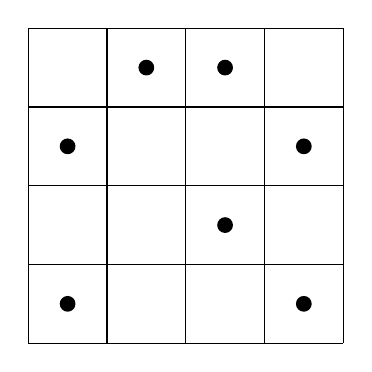
\begin{tikzpicture}
            \draw[step=1cm] (0,0) grid (4,4);
            \foreach \x/\y in {0/0,1/3,2/3,3/2,2/1,3/0,0/2} {
                \fill[black] ({\x+0.5},{\y+0.5}) circle (0.1cm);
            }
        \end{tikzpicture}
        \caption{系统随机布点法}
    \end{subfigure}
    \hfill
    \begin{subfigure}[h]{0.3\textwidth}
        \centering
        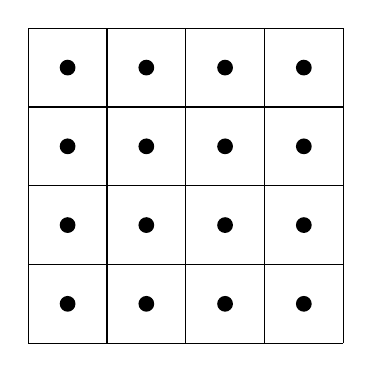
\begin{tikzpicture}
            \draw[step=1cm] (0,0) grid (4,4);
            \foreach \x in {0,1,2,3} {
                \foreach \y in {0,1,2,3} {
                    \fill[black] ({\x+0.5},{\y+0.5}) circle (0.1cm);
                }
            }
        \end{tikzpicture}
        \caption{系统布点法}
    \end{subfigure}
    \hfill
    \begin{subfigure}[h]{0.3\textwidth}
        \centering
        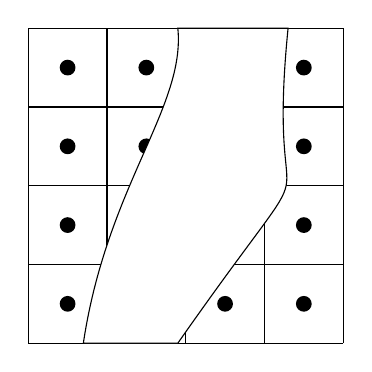
\begin{tikzpicture}
            \draw[step=1cm] (0,0) grid (4,4);
            \foreach \x in {0,1,2,3} {
                \foreach \y in {0,1,2,3} {
                    \fill[black] ({\x+0.5},{\y+0.5}) circle (0.1cm);
                }
            }
            \draw[smooth, fill=white] (0.7,0) .. controls (1,2) and (2,3) .. (1.9,4) -- ++(1.4,0) .. controls (3,1) and (4,3) .. (1.9,0) -- cycle;
        \end{tikzpicture}
        \caption{分区布点法}
    \end{subfigure}
    \caption{监测点位布设方法示意图\cite{HJ25.2-2019}}
    \label{fig:Soil monitoring point layout method (commonly used)}
\end{figure}

如图 \ref{fig:Soil monitoring point layout method (commonly used)} 和表 \ref{tab:Several common distribution methods and applicable conditions} 所示,常用的土壤监测点位布设方法有多种,分别是系统随机布点法、专业判断布点法、系统布点法、分区布点法。考虑到校区实验楼建设项目地块土壤污染特征不明确,则采用系统布点法进行监测点位布设。系统布点法是将监测区域分成面积相等的若干工作单元,每个工作单元内布设一个监测点位。

查阅《建设用地土壤污染风险管控和修复监测技术导则》(HJ 25.2-2019),单个工作单元的面积可根据实际情况确定,原则上不应超过 1600 m$^2$。对于面积较小的地块,应不少于5个工作单元。

\paragraph{$\bullet $ 监测布点图}~{}\par

以成都理工大学宜宾校区实验楼建设为项目例子,查阅中国气象局,四川宜宾的常年风向是东南风和西南风。考虑风向布点如下:
\begin{figure}[H]
    \centering
    \includegraphics[width=\textwidth]{figures/Soil monitoring dot map.png}
    \caption{土壤监测布点图}
    \label{fig:Soil monitoring dot map}
\end{figure}

如图 \ref{fig:Soil monitoring dot map} 所示,一共设置了8个监测点:

在项目建设期间,由于可能产生大气沉降污染,建议在项目占地范围外,根据主导风向的上风向和下风向各设置至少一个表层样本监测点。根据中国气象局的数据显示,四川宜宾地区的常年风向主要为东南风和西南风。因此,在上风向方向应设立一个监测点,而在下风向方向则建议设置两个监测点。这样的设置可以更全面地监测大气沉降污染情况,确保项目对环境的影响能够得到及时有效的评估和控制。
\begin{itemize}
    \item 北上风向监测 $(g104^{\circ}41'22.52'',28^{\circ}49'14.55'')$:选择这个监测点是为了监测来自北方的风向,这样可以了解北方是否存在潜在的污染源,并对风向的变化进行监测。
    \item 西南下风向监测点 $(g104^{\circ}41'14.11'',28^{\circ}48'54.69'')$:选择这个监测点是为了监测来自西南方向的风向。西南下风向是项目占地区域内可能受到污染物影响的方向,监测此处可以提供关于污染物传播的重要信息。
    \item 东南下风向监测点 $(g104^{\circ}41'32.16'',28^{\circ}48'55.64'')$:选择这个监测点是为了监测来自东南方向的风向。东南下风向也是项目占地区域内可能受到污染物影响的方向,监测此处可以提供关于污染物传播的重要信息。
\end{itemize}

针对可能对地面漫流途径产生影响的情况,建议根据地形地貌,在项目占地范围外的上游和下游各设置一个表层样本监测点。然而,鉴于范围内的河流面积相对较小,所以在水流的中点只设置了一个监测点。
这样的监测点布置策略将有助于全面评估地面漫流途径可能带来的影响,并结合地形地貌因素进行合理的监测点位置选择。通过在上游和下游各设置一个监测点,可以有效监测沿水流方向的潜在影响。虽然范围内的河流面积较小,但在水流中点设置监测点可以提供对整体情况的综合评估。
\begin{itemize}
    \item 水流监测点 $(g104^{\circ}41'22.17'',28^{\circ}49'6.93'')$:选择这个监测点是为了监测水流的方向和流速。水流的监测对于了解水体中的污染物传播和扩散非常重要,可以帮助评估污染物对土壤的影响范围。
\end{itemize}

% 系统布点法通常基于以下原则:首先,在区域内选择均匀分布的点,以覆盖整个区域,并保证结果的代表性。其次,考虑到可能存在的污染源或潜在的影响区域,选择在可能受到污染物影响的位置进行监测。点1到点4的选择则是根据这些原则确定的,以确保有效监测土壤中的污染情况。
系统布点法通常基于以下原则进行设计和选择监测点。首先,要确保在区域内选择均匀分布的监测点,以覆盖整个区域并保证结果的代表性。其次,需要考虑潜在的污染源或可能受到污染物影响的区域,以选择适当的监测位置。
在本案例中,点1到点4的选择是基于这些原则确定的,旨在有效监测土壤中的污染情况。通过均匀分布这些监测点,可以全面覆盖整个区域并确保监测结果的可靠性。同时,这些点的位置选择还考虑了可能存在的污染源或潜在的影响区域,以确保对可能受到污染物影响的地区进行监测。
使用系统布点法能够帮助您有效评估土壤污染情况,并为制定相应的环境保护和修复策略提供准确的数据支持。
\begin{itemize}
    \item 点1: $(g104^{\circ}41'20.11'',28^{\circ}49'4.01'')$
    \item 点2: $(g104^{\circ}41'21.78'',28^{\circ}49'5.32'')$
    \item 点3: $(g104^{\circ}41'23.13'',28^{\circ}49'4.24'')$
    \item 点4: $(g104^{\circ}41'21.49'',28^{\circ}49'2.56'')$
\end{itemize}



\subsubsection{监测因子}
\paragraph{$\bullet $ 基本因子}~{}\par
因为土地利用为建设用地,所以遵循《土壤环境质量——建设用地土壤污染风险管控标准(试行)》(GB 36600-2018),然后校园实验楼项目又可以细分为第一类用地:公共管理与公共服务用地中的中小学用地(A33)。根据其中的建设用地土壤污染风险筛选值和管制值(基本项目)表格可以选定三个常规重金属为污染物项目作为土壤环境现状监测基本因子:
\begin{table}[H]
    \centering
    \caption{土壤环境现状监测基本因子\cite{GB36600-2018}}
    \begin{tabular}{cccc}
    \multicolumn{4}{r}{单位:mg/kg} \\
    \toprule
    污染物项目 & CAS 编号 & 筛选值   & 管制值 \\
    \midrule
    铬(六价) & 18540-29-9 & 3.0   & 30 \\
    铜     & 7440-50-8 & 2000  & 8000 \\
    铅     & 7439-92-1 & 400   & 800 \\
    \bottomrule
    \end{tabular}
    \label{tab:Basic factors for monitoring the status of soil environment}
\end{table}

\paragraph{$\bullet $ 特征因子}~{}\par
如表 \ref{tab:Soil environmental impact types and impact pathways of construction projects} 所示,可以设置项目特征因子为大气沉降、地面漫流、垂直入渗的监测因子。



\subsubsection[监测方法]{监测方法\cite{HJ25.2-2019}}
\paragraph{$\bullet $ 表层土壤样品的采集}~{}\par
\begin{enumerate}
    \item 表层土壤样品的采集一般采用挖掘方式进行,一般采用锹、铲及竹片等简单工具,也可进行钻孔取样。
    \item 土壤采样的基本要求为尽量减少土壤扰动,保证土壤样品在采样过程不被二次污染。
\end{enumerate}

\paragraph{$\bullet $ 下层土壤样品的采集}~{}\par
\begin{enumerate}
    \item 下层土壤的采集以钻孔取样为主,也可采用槽探的方式进行采样。
    \item 钻孔取样可米用人上心螺旅钻、中空螺旋钻、套管钻等。据他断而管式采样器等。机械钻探包括实心螺旋钻、中空螺旋钻、套管钻等。
    \item 槽探一般靠人工或机械挖掘采样槽,然后用采样铲或采样刀进行采样。槽探的断面呈长条形,根据地块类型和采样数量设置一定的断面宽度。槽探取样可通过锤击敞口取土器取样和人工刻切块状土取样。
\end{enumerate}

\paragraph{$\bullet $ 下层土壤样品的采集}~{}\par
挥发性有机物污染、易分解有机物污染、恶臭污染土壤的采样,应采用无扰动式的采样方法和工具。钻孔取样可采样快速击入法、快速压入法及回转法,主要工具包括土壤原状取土器和回转取土器。槽探可采用人工刻切块状土取样。采样后立即将样品装入密封的容器,以减少暴露时间。

\paragraph{$\bullet $ 土壤混合样的采集}~{}\par
如需采集土壤混合样时,将等量各点采集的土壤样品充分混拌后四分法取得到土壤混合样。含易挥发、易分解和恶臭污染的样品必须进行单独采样,禁止对样品进行均质化处理,不得采集混合样。

\paragraph{$\bullet $ 土壤样品的保存与流转}~{}\par
\begin{enumerate}
    \item 挥发性有机物污染的土壤样品和恶臭污染土壤的样品应采用密封性的采样瓶封装,样品应充满容器整个空间;含易分解有机物的待测定样品,可采取适当的封闭措施(如甲醇或水液封等方式保存于采样瓶中)。样品应置于4℃以下的低温环境(如冰箱)中运输、保存,避免运输、保存过程中的挥发损失,送至实验室后应尽快分析测试。
    \item 挥发性有机物浓度较高的样品装瓶后应密封在塑料袋中,避免交叉污染,应通过运输空白样来控制运输和保存过程中交叉污染情况。
    \item 具体土壤样品的保存与流转应按照 HJ/T 166的要求进行。
\end{enumerate}

\paragraph{$\bullet $ 土壤样品分析}~{}\par
土壤样品关注污染物的分析测试应参照 GB 36600 和 HJ/T 166 中的指定方法。土壤的
常规理化特征土壤 pH、粒径分布、密度、孔隙度、有机质含量、渗透系数、阳离子交换量
等的分析测试应按照 GB 50021 执行。污染土壤的危险废物特征鉴别分析,应按照 GB 5085
和 HJ 298 中的指定方法。

\paragraph{$\bullet $ 监测因子分析方法}~{}\par
\begin{table}[H]
    \centering
    \caption{土壤污染物分析方法}
    \begin{tabular}{ccc}
    \toprule
    污染物项目  & 分析方法  & 标准编号 \\
    \midrule
    铬(六价)  & 火焰原子吸收分光光度法 & HJ 491-2019 \\
    铜      & 火焰原子吸收分光光度法 & HJ 491-2019 \\
    铅     & 火焰原子吸收分光光度法 & HJ 491-2019 \\
    \bottomrule
    \end{tabular}
    \label{tab:Methods for soil pollutant analysis}
\end{table}



\subsubsection{监测时期}

根据《土壤环境监测技术规范》(HJ/T 166-2004)要求,可以选定监测时期为污染物更为容易扩散的夏季。

\begin{table}[H]
    \centering
    \caption{土壤监测项目与监测频次\cite{HJ/T166-2004}}
    \begin{tabular}{|c|c|c|c|}
    \hline
    \multicolumn{2}{|c|}{项目类别} & 监测项目  & 监测频次 \\
    \hline
    \multirow{2}*{常规项目} & 基本项目  & pH、阳离子交换量 & \multirow{2}*{\makecell[l]{每3年一次\\农田在夏收或秋收后采样}} \\
    \cline{2-3}          & 重点项目  &  \makecell[l]{镉、铬、汞、砷、铅、铜、\\锌、镍、六六六、滴滴涕} &  \\
    \hline
    \multicolumn{2}{|c|}{特定项目(污染事故)} & 特征项目  & \makecell[l]{及时采样,根据污染物\\变化趋势决定监测频次} \\
    \hline
    \end{tabular}
    \label{tab:Soil monitoring projects and monitoring frequency}
\end{table}
  



\subsubsection{监测次数}
\begin{enumerate}
    \item 基本因子:该建设项目的评价工作等级为为二级,每3年至少1次的监测数据;
    %引用监测数据应满足7.4.2和7.4.3的相关要求,并说明数据有效性;
    \item 特征因子:应至少开展1次现状监测。
\end{enumerate}



\subsection{小结及建议}

制定某校区实验楼建设项目的土壤环境质量现状监测方案是确保项目建设与环境保护的重要环节。通过科学合理的监测方案,可以及时发现和评估土壤环境质量变化情况,采取相应的措施保护土壤资源和生态环境。

在上面的现状监测方案制定中,提出了确定监测范围、布点设计、监测因子、监测方法、监测时期和次数等关键步骤和考虑因素。这些措施将有助于评估实验楼建设对土壤环境的影响,及时采取相应的保护和修复措施。同时,强调了代表性和充分覆盖原则在布点设计中的重要性,以确保监测结果的可靠性和代表性。

最后,制定和执行土壤环境质量现状监测方案应与相关法律法规和标准保持一致,确保建设项目符合环境保护的要求,为校区实验楼建设提供科学依据和环境保障。

 % 实验三部分 土
\newpage\null\par
\section{实验四\hspace{1em}声环境质量现状评价}
\subsection{教学目的与要求}
\noindent\textbf{教学目的:}通过噪声源参数现状数据实例来进行声环境质量评价。

\noindent\textbf{教学要求:}
\begin{enumerate}
    \item 掌握声环境质量现状调查监测计划的设置方法,制定某校区的声环境质量现状监测方案并进行评价;
    \item 掌握声环境预测软件EIAN2.0和Surfer绘图软件在声环境质量评价中的应用,熟悉等声值线图绘制的基本方法。利用EIAN和Sufer软件自行拟定参数(声源分贝、预测网格步长等)绘制出一个声源(点源或者面源)的分布衰减等声线图(图形优化后),并附上主要操作步骤截图。
    \item 鼓励使用Cadna/A 软件进行影响预测。
\end{enumerate}


\subsection{实验报告背景}
\subsubsection{监测点布设}
监测点布设本项目噪声监测共布设4个点(如图 \ref{fig:Acoustic environment monitoring dot map}、\ref{fig:Sound_environment_monitoring_points} 和表 \ref{tab:Acoustic environment monitoring location information} 所示)。按国家规定的噪声测试规范要求进行昼间和夜间环境噪声监测。

\begin{table}[H]
    \centering
    \caption{声环境监测布点位置信息}
    \begin{tabular}{cccc}
        \toprule
        图像点位 & 位置名称 & 经度 & 纬度 \\
        \midrule
        点1 & 体育馆二楼篮球场 & $104^{\circ}41'26.58''$ & $28^{\circ}48'58.51''$ \\
        点2 & 图书馆二楼中心 & $104^{\circ}41'32.01''$ & $28^{\circ}49'3.43''$ \\
        点3 & 教学楼甲一楼 & $104^{\circ}41'32.88''$ & $28^{\circ}49'7.96''$ \\
        点4 & 一期食堂一楼 & $104^{\circ}41'40.11''$ & $28^{\circ}48'59.28''$ \\
        \bottomrule
    \end{tabular}
    \label{tab:Acoustic environment monitoring location information}
\end{table}

\begin{figure}[H]
    \centering
    \includegraphics[width=\textwidth]{figures/Acoustic environment monitoring dot map.png}
    \caption{声环境监测布点图}
    \label{fig:Acoustic environment monitoring dot map}
\end{figure}

\begin{figure}[H]
    \centering
    \begin{subfigure}[htb]{0.48\textwidth}
        \centering
        \includegraphics[width=\textwidth]{figures/Monitoring_point_-_basketball_court_on_the_second_floor_of_the_gymnasium.jpg}
        \caption{体育馆二楼篮球场}
    \end{subfigure}
    \hfill
    \begin{subfigure}[htb]{0.48\textwidth}
        \centering
        \includegraphics[width=\textwidth]{figures/Monitoring_point_-_center_on_the_second_floor_of_the_library.jpg}
        \caption{图书馆二楼中心}
    \end{subfigure}
    \hfill
    \begin{subfigure}[htb]{0.48\textwidth}
        \centering
        \includegraphics[width=\textwidth]{figures/Monitoring_point_-_the_first_floor_of_the_teaching_building.jpg}
        \caption{教学楼甲一楼}
    \end{subfigure}
    \hfill
    \begin{subfigure}[htb]{0.48\textwidth}
        \centering
        \includegraphics[width=\textwidth]{figures/Monitoring_point_-_the_first_floor_of_the_canteen_of_the_first_phase.jpg}
        \caption{一期食堂一楼}
    \end{subfigure}
    \caption{声环境监测点实时图}
    \label{fig:Sound_environment_monitoring_points}
\end{figure}


\subsubsection{监测项目说明}
\paragraph{$\bullet$ 监测时段}~{}\par
分别测定昼间和夜间的等效A声级,连续监测2天,昼、夜间各一次。

\begin{sidewaystable}[p]
    \centering
    \caption{声环境监测数据}
    \resizebox{\textwidth}{!}{
    \begin{tabular}{|c|c|c|c|c|c|c|c|c|c|c|c|c|c|c|c|}
    \multicolumn{16}{r}{单位:dB(A)} \\
    \hline
    \textbf{地点} & \textbf{时间} & \textbf{监测日期} & \textbf{风向} & \textbf{风速km/h} & \textbf{天气} & \textbf{Leq} & \textbf{SEL} & \textbf{Lmax} & \textbf{Lmin} & \textbf{L5} & \textbf{L10} & \textbf{L50} & \textbf{L90} & \textbf{L95} & \textbf{SD} \\
    \hline
    \multirow{4}*{教学楼甲一楼} & \multirow{2}*{$9:00-10:00$} & 2023/6/7 & 东北    & 2     & 晴     & 54.1  & 89.7  & 79.0  & 33.2  & 58.8  & 53.8  & 41.2  & 36.8  & 35.8  & 7.1  \\
    \cline{3-16}          &       & 2023/6/8 & 东北    & 6     & 小雨    & 51.9  & 87.5  & 80.1  & 32.8  & 56.0  & 50.2  & 38.8  & 34.8  & 34.4  & 6.7  \\
    \cline{2-16}          & \multirow{2}*{$19:30-20:30$} & 2023/6/6 & 西     & 4     & 晴     & 50.2  & 85.8  & 80.7  & 31.4  & 45.6  & 42.0  & 37.0  & 34.6  & 33.8  & 4.3  \\
    \cline{3-16}          &       & 2023/6/7 & 北     & 4     & 晴     & 52.6  & 88.2  & 79.1  & 33.6  & 55.6  & 51.4  & 43.0  & 37.2  & 36.4  & 6.1  \\
    \hline
    \multirow{4}*{体育馆二楼篮球场} & \multirow{2}*{$10:30-11:30$} & 2023/6/7 & 东     & 2     & 晴     & 70.4  & 106.0  & 96.8  & 53.5  & 74.2  & 72.8  & 68.6  & 64.2  & 62.8  & 3.5  \\
    \cline{3-16}          &       & 2023/6/8 & 东北    & 6     & 小雨转阴  & 69.8  & 105.4  & 88.8  & 56.3  & 73.0  & 72.2  & 69.2  & 66.0  & 65.0  & 2.4  \\
    \cline{2-16}          & \multirow{2}*{$20:00-21:00$} & 2023/6/6 & 西北    & 4     & 晴     & 68.8  & 104.4  & 89.8  & 51.8  & 73.4  & 71.4  & 66.4  & 61.8  & 60.6  & 3.9  \\
    \cline{3-16}          &       & 2023/6/7 & 北     & 4     & 晴     & 65.7  & 101.3  & 88.1  & 44.0  & 70.8  & 69.0  & 63.2  & 57.8  & 56.2  & 4.4  \\
    \hline
    \multirow{4}*{图书馆二楼中心} & \multirow{2}*{$9:30-10:30$} & 2023/6/7 & 东     & 2     & 晴     & 42.8  & 78.4  & 59.0    & 29.9  & 48.8  & 46.6  & 38.8  & 33.6  & 32.6  & 4.9 \\
    \cline{3-16}          &       & 2023/6/8 & 东北    & 6     & 小雨    & 43.8  & 79.4  & 73.7  & 28.9  & 48.2  & 45.8  & 38.2  & 32.8  & 31.8  & 5.0 \\
    \cline{2-16}          & \multirow{2}*{$21:00-22:00$} & 2023/6/6 & 北     & 5     & 晴     & 49.2  & 84.8  & 80.1  & 45.2  & 51.0    & 49.0  & 47.4  & 46.8  & 46.6  & 1.6 \\
    \cline{3-16}          &       & 2023/6/7 & 北     & 4     & 晴     & 43.6  & 79.2  & 66.0  & 30.1  & 50.6  & 44.6  & 37.2  & 33.4  & 32.6  & 5.1 \\
    \hline
    \multirow{4}*{一期食堂一楼} & \multirow{2}*{$11:30-12:30$} & 2023/6/7 & 东南    & 2     & 晴     & 68.8  & 104.4 & 82.1  & 63.1  & 71.6  & 70.8  & 68.2  & 66.0  & 65.4  & 1.9 \\
    \cline{3-16}          &       & 2023/6/8 & 东北    & 10    & 小雨转阴  & 68.6  & 104.2 & 83.7  & 63.0  & 71.4  & 70.6  & 68.0  & 65.8  & 65.2  & 1.8 \\
    \cline{2-16}          & \multirow{2}*{$22:00-23:00$} & 2023/6/6 & 北     & 3     & 晴     & 52.3  & 87.2  & 89.5  & 41.8  & 53.6  & 51.2  & 46.8  & 44.4  & 44.0  & 3.4 \\
    \cline{3-16}          &       & 2023/6/7 & 北     & 4     & 晴     & 50.2  & 85.8  & 69.0  & 39.7  & 54.6  & 53.2  & 48.6  & 43.2  & 42.2  & 3.8 \\
    \hline
    \end{tabular}}
    \label{tab:Summary of monitoring records}
\end{sidewaystable}


\paragraph{$\bullet$ 监测方法及数据统计}~{}\par
使用AWA5688多功能声级计,按标准规范执行,即按《社会生活环境噪声排放标准》(GB 22337-2008)进行测量。监测各测点处的连续等效A声级。


\paragraph{$\bullet$ 数据处理}~{}\par
按国家标准方法和推荐方法进行,提供$\mathrm{L_{Aeq}}$值。
环境噪声评价量,等效声级 $\mathrm{L_{eq}}$ 计算公式:
\begin{equation} \label{eq:how to get Leq}
	\mathrm{L_{eq}} = 10\lg{\dfrac{1}{N}\sum^N_{i=1}10^{0.1L_i}}
\end{equation}
式中:$L_i$——第 $i$ 次读取的A声级;\newline
\phantom{式中:}$N$——取样总数。

将数据按顺序排列找出 $\mathrm{L_{5}}$、$\mathrm{L_{10}}$、$\mathrm{L_{50}}$、$\mathrm{L_{90}}$、$\mathrm{L_{95}}$,
并计算出噪声标准差 SD :
\begin{equation}
    \text{{SD}} = \sqrt{\frac{1}{N}\sum_{i=1}^{N}(X_i - \bar{X})^2}
\end{equation}
其中,$N$表示样本的数量; \\
\phantom{其中,}$X_i$表示第$i$个样本值; \\
\phantom{其中,}$\bar{X}$表示样本均值。

因为监测的时间为1小时 $T=3600$ s,所以可以计算出暴露声压级:
\begin{align}
    \text{SEL} &= \mathrm{L_{eq}} + 10\lg{(T)} \\
    &= \mathrm{L_{eq}} + 10\lg{(3600)} \notag
\end{align}

点声源的几何发散衰减计算公式:
\begin{align} \label{eq:Geometric divergence attenuation calculation of point sound sources}
    % A_{div} = 10\lg{\dfrac{1}{4\pi r^2}} \\
    A_{div} = 20\lg{\dfrac{r}{r_0}}
\end{align}
式中:$A_{div}$——几何发散引起的衰减,dB;\\
\phantom{式中:}$r$——预测点距声源的距离;\\
\phantom{式中:}$r_0$——参考位置距声源的距离。

 

\subsubsection{监测评价相关标准}
% \begin{itemize}
%     \item 《声环境质量标准》( GB 3096-2008)
%     \item 《社会生活环境噪声排放标准》( GB 22337-2008)
%     \item 《环境影响评价技术导则——声环境》( HJ 2.2-2018)
% \end{itemize}

根据《声环境质量标准》( GB 3096-2008)声环境功能区分类标准,按照区域的使用功能特点和环境质量要求,将声环境功能区划分为五种类型:
\begin{enumerate}[label={\arabic*类声环境功能区:},align=left, leftmargin=*]
    \setcounter{enumi}{-1}
    \item 指康复疗养区等特别需要安静的区域。
    \item 指以居民住宅、医疗卫生、文化教育、科研设计、行政办公为主要功能,需要保持安静的区域。
    \item 指以商业金融、集市贸易为主要功能,或者居住、商业、工混杂,需要维护住宅安静的区域。
    \item 指以工业生产、仓储物流为主要功能,需要防止工业噪声对周围环境产生严重影响的区域。
    \item 指交通干线两侧一定区域之内,需要防止交通噪声对周围环境产生严重影响的区域,包括4a类和4b类两种类型。4a类为高速公路、一级公路、二级公路、城市快速路、城市主干路、城市次干路、城市轨道交通(地面段)、内河航道两侧区域;4b类为铁路干线两侧区域。
\end{enumerate}

\begin{table}[H]
    \centering
    \caption{环境噪声限值\cite{GB3096-2008}}
    \begin{tabular}{|c|c|c|c|}
        \multicolumn{4}{r}{单位:dB(A)} \\
        \hline
        \multicolumn{2}{|c|}{\multirow{2}*{\hspace{2em}声环境功能区类别\hspace{2em}}} & \multicolumn{2}{c|}{时段} \\
        \cline{3-4}    \multicolumn{2}{|c|}{} & \hspace{2em}昼间\hspace{2em}    & \hspace{2em}夜间\hspace{2em} \\
        \hline
        \multicolumn{2}{|c|}{0类} & 50    & 40 \\
        \hline
        \multicolumn{2}{|c|}{1类} & 55    & 45 \\
        \hline
        \multicolumn{2}{|c|}{2类} & 60    & 50 \\
        \hline
        \multicolumn{2}{|c|}{3类} & 65    & 55 \\
        \hline
        \multirow{2}*{\hspace{2em}4类\hspace{2em}} & 4a类   & 70    & 55 \\
        \cline{2-4} & 4b类   & 70    & 60 \\
        \hline
    \end{tabular}
    \label{tab:Ambient noise limits}
\end{table}

由于我们选择的监测点位于校园的文化教育区域,因此根据声环境功能区的分类,这些点属于1类声环境功能区。所以环境噪声限值为:
$\text{昼间}\leqslant 55 \;\mathrm{dB(A)}$,$\text{夜间}\leqslant 45 \;\mathrm{dB(A)}$。


\subsection{报告主体部分}

\subsubsection{数据加工}

因为声环境监测方案选定了一个地点选定昼夜两次,连续两天(见表 \ref{tab:Summary of monitoring records})。所以在进行相同时段分析的时候,根据公式 \ref{eq:how to get Leq} 计算出同时段等效声级如下表所示:

\begin{table}[H]
    \centering
    \caption{同时段等效声级}
    \begin{tabular}{|c|c|c|c|}
    \hline
    \textbf{地点} & \textbf{昼夜} & \textbf{计算过程} & \textbf{同时段等效声级 dB(A)} \\\hline
    \multirow{2}*{教学楼甲一楼} & 昼  & $10\lg{(10^{5.41}+10^{5.19})/2}$  & 53.14  \\\cline{2-4}
            & 夜  & $10\lg{(10^{5.02}+10^{5.26})/2}$   & 51.56  \\\hline
    \multirow{2}*{体育馆二楼篮球场} & 昼  & $10\lg{(10^{7.04}+10^{6.98})/2}$   & 70.11  \\\cline{2-4}
            & 夜  & $10\lg{(10^{6.88}+10^{6.57})/2}$   & 67.52  \\\hline
    \multirow{2}*{图书馆二楼中心} & 昼  & $10\lg{(10^{4.28}+10^{4.38})/2}$   & 43.33  \\\cline{2-4}
            & 夜  & $10\lg{(10^{4.92}+10^{4.36})/2}$   & 47.25  \\\hline
    \multirow{2}*{一期食堂一楼} & 昼  & $10\lg{(10^{6.88}+10^{6.86})/2}$   & 68.70  \\\cline{2-4}
            & 夜  & $10\lg{(10^{5.23}+10^{5.02})/2}$   & 51.38  \\\hline
    \end{tabular}
    \label{tab:Equivalent sound levels in the same segment}
\end{table}
  
这几天平均昼间温度为 25℃,相对湿度为 80\%;夜间温度为 25℃,相对湿度为 80\%。则可以通过EIAN和Sufer两个软件进行衰减预测,绘制不同点源分布的衰减等声线图。


\subsubsection{EIAN 2.0 操作步骤}
\begin{enumerate}
    \item 文件 $\rightarrow $ 背景图形文件 $\rightarrow $ 插入图形 $\rightarrow $ 定义两个点
    \begin{enumerate}[label=\arabic*)]
        \item 在奥维互动地图中找到合适的俯视全景图,想办法导出 .jpg 格式的图片文件,然后插入背景图片;
        \begin{figure}[H]
            \centering
            \includegraphics[width=0.8\textwidth]{figures/acoustic_step1.png}
            \caption{插入背景图形文件}
        \end{figure}

        \item 定义第一点:体育馆二楼篮球场 $(0,0)$ ;
        \item 定义第二点:图书馆二楼中心 $(220,0)$ ;
        \item 设置实际距离为 228 m。
    \end{enumerate}
    
    \item 衰减计算 $\rightarrow $ 噪声衰减分布计算 $\rightarrow $ 声源属性
    \begin{enumerate}[label=\arabic*)]
        \item 设置一般属性(名称、坐标、声源离地面高度);
        \begin{itemize}
            \item 体育馆二楼篮球场:坐标 $(0,0)$,高度为 5 m
            \item 图书馆二楼中心:坐标 $(220,0)$,高度为 1 m
            \item 教学楼甲一楼:坐标 $(339,84)$,高度为 1 m
            \item 一期食堂一楼:坐标 $(291,-242)$,高度为 1 m
        \end{itemize}
        \begin{figure}[H]
            \centering
            \includegraphics[width=0.8\textwidth]{figures/acoustic_step2-1.png}
            \caption{一般属性}
        \end{figure}

        \item 因为总声功率级为A计权,所以设置发声特性中总的声功率级的代表频率都为 1000 Hz。因此,只需要设置各噪声源总的声功率级(或A声功率级)。
        \begin{itemize}
            \item 体育馆二楼篮球场(昼/夜):70.11/67.52 dB(A)
            \item 图书馆二楼中心(昼/夜):43.33/47.25 dB(A)
            \item 教学楼甲一楼(昼/夜):53.14/51.56 dB(A)
            \item 一期食堂一楼(昼/夜):68.70/51.38 dB(A)
        \end{itemize}
        \begin{figure}[H]
            \centering
            \includegraphics[width=0.8\textwidth]{figures/acoustic_step2-2.png}
            \caption{发声特性}
        \end{figure}
    \end{enumerate}
    
    \item 噪声衰减分布计算 $\rightarrow $ 预测方案属性
    \begin{enumerate}[label=\arabic*)]
        \item 选择“从背景图形上取得坐标”,然后画出来预测范围;
        \begin{figure}[H]
            \centering
            \includegraphics[width=0.8\textwidth]{figures/acoustic_step3-1.png}
            \caption{框选预测范围}
        \end{figure}

        \item 设置环境空气参数;
        \begin{itemize}
            \item 环境空气温度:25 ℃
            \item 空气相对湿度:80 \%
            \item 空气大气压:1 atm
        \end{itemize}
        \item 预测点X坐标与Y坐标的步长,默认值是100m,画出的图形为趋势图,这里调整为10m;
        \item 预测结果选项全部勾选。
        \begin{itemize}
            \item 考虚虑空气吸收的衰减量
            \item 考虑地面吸收的衰减量
        \end{itemize}
        \begin{figure}[H]
            \centering
            \includegraphics[width=0.8\textwidth]{figures/acoustic_step3-2.png}
            \caption{预测属性修改}
        \end{figure}
    \end{enumerate}

    \item 噪声衰减分布计算 $\rightarrow $ 预测结果 $\rightarrow $ 刷新结果
    \begin{figure}[H]
        \centering
        \includegraphics[width=0.8\textwidth]{figures/acoustic_step4.png}
        \caption{生成噪声衰减结果}
        \label{fig:Generate noise attenuation results}
    \end{figure}
    刷新得到的预测结果复制保存到.txt文件或者Excel文件中,为之后使用Sufer软件绘图提供噪声衰减数据。

    \item 预测结果 $\rightarrow $ 绘图 $\rightarrow $ A计权声级dB(A)
    % \begin{figure}[H]
    %     \centering
    %     \includegraphics[width=0.8\textwidth]{figures/acoustic_step5.png}
    %     \caption{绘制A计权声级图}
    % \end{figure}

    \item 最后,生成昼夜两个时段的校园噪声衰减图:
    \begin{figure}[H]
        \centering
        \begin{subfigure}[h]{\textwidth}
            \centering
            % \includegraphics[width=0.8\textwidth]{figures/acoustic_step6-1.png}
            \includegraphics[width=0.8\textwidth]{figures/Campus noise attenuation plot-daytime.jpg}
            \caption{昼}
        \end{subfigure}
        \hfill
        \begin{subfigure}[h]{\textwidth}
            \centering
            % \includegraphics[width=0.8\textwidth]{figures/acoustic_step6-2.png}
            \includegraphics[width=0.8\textwidth]{figures/Campus noise attenuation plot-nighttime.jpg}
            \caption{夜}
        \end{subfigure}
        \caption{EIAN-校园噪声衰减图}
    \end{figure}
\end{enumerate}


\subsubsection{SCV 文件生成}
将生成的噪声衰减结果(如图 \ref{fig:Generate noise attenuation results})复制并保存到Excel中,然后将其转换为Sufer软件要求的导入格式(A列应包含X坐标,B列应包含Y坐标,C列应包含相应的噪声衰减值),就可以开始绘制噪声衰减图了。

\begin{figure}[H]
    \centering
    \begin{tikzpicture}
        \draw (1.2,0) rectangle node[midway] {$X$} (4,-1);
        \draw (0,-1.2) rectangle node[midway] {$Y$} (1,-4);
        \draw (1.2,-1.2) rectangle node[midway] {$Z$} (4,-4);
        \node[above] at (2,0.2) {原数据格式};
    \end{tikzpicture}
    \quad
    \tikz\draw[-stealth] (0,0) ++(0,2) -- ++(2,0) node[midway, above] {转换};
    \quad
    \begin{tikzpicture}
        \draw (0,0) rectangle node[midway] {$X$} (1,-4);
        \draw (1.2,0) rectangle node[midway] {$Y$} (2.2,-4);
        \draw (2.4,0) rectangle node[midway] {$Z$} (3.4,-4);
        \node[above] at (1.7,0.2) {目标CSV格式};
    \end{tikzpicture}
\end{figure}

由于在选择预测范围时选择了较大的区域:$(-94, -314)$ 到 $(552, 272)$,并且步长设置为每隔10米生成一次计算结果,所以最终得到的噪声衰减结果会非常庞大,数据总数为$X \times Y = 66 \times 60 = 3960$个。手动复制和粘贴来修改这么多数据的格式将会非常繁琐,因此我编写了一个小的Python程序来完成这个格式转化的任务。

\begin{lstlisting}[caption={将excel数据按要求转为csv.py}, label={lst:python_code}]
import pandas as pd
import csv

def extract_data(excel_file, sheet_index, csv_filename):
    # 提取数据和标题
    data = excel_file.parse(excel_file.sheet_names[sheet_index], header=0, index_col=0)
    x_title = data.columns.tolist()  # X坐标数组
    y_title = data.index.tolist()  # Y坐标数组
    data_values = data.values.tolist()  # 坐标值Z二维数组
    # 重新排列数据
    xyz = [[], [], []]
    for x in x_title:
        xyz[0].extend([x] * len(y_title))  # 录入X坐标
        xyz[1].extend(y_title)  # 录入Y坐标
        for each in range(len(data_values)):  # 录入相应坐标(X,Y)的Z值
            xyz[2].append(data_values[each][x_title.index(x)])
    # 创建CSV文件并写入数据
    with open(csv_filename, 'w', newline='') as csvfile:
        writer = csv.writer(csvfile)
        for row in zip(*xyz):
            writer.writerow(row)  # 列向写入数据
    print(csv_filename, "已生成CSV文件!")

# 读取Excel文件,并提取两个工作表(昼/夜)的数据
excel_file = pd.ExcelFile('校园噪声衰减数据.xlsx')  # Excel文件与.py路径同源
extract_data(excel_file, 0, 'daytime_xyz.csv')
extract_data(excel_file, 1, 'nighttime_xyz.csv')    
\end{lstlisting}

运行上述代码,我得到了 daytime_xyz.csv 和 nighttime_xyz.csv 文件,那么就可以开始下一步: Sufer 软件的使用。


\subsubsection{Sufer 操作步骤}
\begin{enumerate}
    \item Surfer 预处理生成 .grd 文件
    \begin{enumerate}[label=\arabic*)]
        \item 网格 $\rightarrow $ 数据 $\rightarrow $ 打开生成的 csv 文件;
        \begin{figure}[H]
            \centering
            \includegraphics[width=0.8\textwidth]{figures/Sufer_step1-1.png}
            \caption{打开生成的 csv 文件}
        \end{figure}
        \item 网格化数据的导入(默认即可)。
        \begin{figure}[H]
            \centering
            \includegraphics[width=0.8\textwidth]{figures/Sufer_step1-2.png}
            \caption{网格化数据导入设置}
        \end{figure}
    \end{enumerate}

    \item 画等值线图
    \begin{enumerate}[label=\arabic*)]
        \item 地图 $\rightarrow $ 等值线图 $\rightarrow $ 新建等值线图;
        \item 打开网格数据,选择刚才用 Excel 生成的 .grd 数据;
        \begin{figure}[H]
            \centering
            \includegraphics[width=0.8\textwidth]{figures/Sufer_step2-1.png}
            \caption{导入 .grd 数据}
        \end{figure}
        \item 一张朴实无华的等值线图就绘制完成。
        \begin{figure}[H]
            \centering
            \includegraphics[width=0.8\textwidth]{figures/Sufer_step2-2.png}
            \caption{初始样式等声值线图}
        \end{figure}
    \end{enumerate}

    \item 等声值线图优化
    \begin{enumerate}[label=\arabic*)]
        \item 右键点击图片,打开“属性”;
        \item 依次将填充等值线和平滑中的选项勾选:
        \begin{itemize}
            \item 填充等值线(F)
            \item 平滑等值线(s)
            \item 颜色比例(C)
            \item 程度(M):高
        \end{itemize}
        \begin{figure}[H]
            \centering
            \includegraphics[width=0.8\textwidth]{figures/Sufer_step3-1.png}
            \caption{修改常规数值}
        \end{figure}

        \item 等级 $\rightarrow $ 填充
        \begin{itemize}
            \item 前景色: White \fcolorbox{black}{white}{\phantom{None}} Blue Violet \fcolorbox{black}{blueviolet}{\phantom{None}}
            \item 其余保持默认
        \end{itemize}
        \begin{figure}[H]
            \centering
            \includegraphics[width=0.8\textwidth]{figures/Sufer_step3-2.png}
            \caption{修改图形颜色}
        \end{figure}

        \item 等级 $\rightarrow $ 等级
        \begin{itemize}
            \item 间距:3
            \item 其余保持默认
        \end{itemize}
        \begin{figure}[H]
            \centering
            \includegraphics[width=0.8\textwidth]{figures/Sufer_step3-3.png}
            \caption{修改等级间距}
        \end{figure}

        \item 完成优化,获得一张全新而又优美且富有个人特色的等声值线图。
        \begin{figure}[H]
            \centering
            \begin{subfigure}[h]{\textwidth}
                \centering
                \includegraphics[width=0.8\textwidth]{figures/Campus noise attenuation plot-daytime.png}
                \caption{昼}
            \end{subfigure}
            \begin{subfigure}[h]{\textwidth}
                \centering
                \includegraphics[width=0.8\textwidth]{figures/Campus noise attenuation plot-nighttime.png}
                \caption{夜}
            \end{subfigure}
            \caption{Sufer-校园昼夜噪声衰减等声值线图}
            \label{fig:Sufer-Isoacoustic line diagram of campus day and night noise attenuation}
        \end{figure}
    \end{enumerate}
\end{enumerate}


\subsubsection{评价分析}
由公式 \ref{eq:Geometric divergence attenuation calculation of point sound sources} 可得,当已知几何发散引起的衰减 $A_{div}$ dB(A),则可以反向求得衰减距离:
\begin{equation}
    r = r_0 \cdot 10^{0.05A}
\end{equation}
因为声环境监测记录的参考位置距声源的距离为 $r_0 = 1$ m,则
\begin{align*}
    r = 10^{0.05A}
\end{align*}
再根据表 \ref{tab:Summary of monitoring records} 中的数据和表 \ref{tab:Ambient noise limits} 中的环境噪声限值,可以计算出噪声达标距离,如下表 \ref{tab:Attenuation attainment distance} 所示:
\begin{table}[H]
    \centering
    \caption{衰减达标距离}
    \resizebox{\textwidth}{!}{
    \begin{tabular}{|c|c|c|c|c|c|c|}
    \multicolumn{7}{r}{单位:dB(A)} \\
    \hline
    \textbf{地点} & \textbf{时间} & \textbf{监测日期} & \textbf{昼夜} & \textbf{标准限值} & \textbf{Leq} & \textbf{衰减达标(m)} \\
    \hline
    \multirow{4}*{教学楼甲一楼} & \multirow{2}*{$9:00-10:00$} & 2023/6/7 & 昼     & 55.0  & 54.1  &  \\
    \cline{3-7}          &       & 2023/6/8 & 昼     & 55.0  & 51.9  &  \\
    \cline{2-7}          & \multirow{2}*{$19:30-20:30$} & 2023/6/6 & 夜     & 45.0  & 50.2  & 1.820  \\
    \cline{3-7}          &       & 2023/6/7 & 夜     & 45.0  & 52.6  & 2.399  \\
    \hline
    \multirow{4}*{体育馆二楼篮球场} & \multirow{2}*{$10:30-11:30$} & 2023/6/7 & 昼     & 55.0  & 70.4  & 5.888  \\
    \cline{3-7}          &       & 2023/6/8 & 昼     & 55.0  & 69.8  & 5.495  \\
    \cline{2-7}          & \multirow{2}*{$20:00-21:00$} & 2023/6/6 & 夜     & 45.0  & 68.8  & 15.488 \\
    \cline{3-7}          &       & 2023/6/7 & 夜     & 45.0  & 65.7  & 10.839 \\
    \hline
    \multirow{4}*{图书馆二楼中心} & \multirow{2}*{$9:30-10:30$} & 2023/6/7 & 昼     & 55.0  & 42.8  &  \\
    \cline{3-7}          &       & 2023/6/8 & 昼     & 55.0  & 43.8  &  \\
    \cline{2-7}          & \multirow{2}*{$21:00-22:00$} & 2023/6/6 & 夜     & 45.0  & 49.2  & 1.622\footnotemark  \\
    \cline{3-7}          &       & 2023/6/7 & 夜     & 45.0  & 43.6  &  \\
    \hline
    \multirow{4}*{一期食堂一楼} & \multirow{2}*{$11:30-12:30$} & 2023/6/7 & 昼     & 55.0  & 68.8  & 4.898  \\
    \cline{3-7}          &       & 2023/6/8 & 昼     & 55.0  & 68.6  & 4.786 \\
    \cline{2-7}          & \multirow{2}*{$22:00-23:00$} & 2023/6/6 & 夜     & 45.0  & 52.3  & 2.317  \\
    \cline{3-7}          &       & 2023/6/7 & 夜     & 45.0  & 50.2  & 1.820  \\
    \hline
    \end{tabular}}
    \label{tab:Attenuation attainment distance}
\end{table}
\footnotetext{由于2023年6月6日当天气温较高,图书馆在晚上开启了空调系统,这一举措旨在为人们提供舒适的环境。然而,由于空调系统的运行,从21:00至22:00期间记录的等效A声级Leq与随后在2023年6月7日晚上进行的监测结果相比较高。这差异也成为了超过标准限值范围的直接原因。}


根据图 \ref{fig:Sufer-Isoacoustic line diagram of campus day and night noise attenuation} 所示,
昼间时,体育馆二楼篮球场和一期食堂一楼对周围环境的影响最为显著,其辐射范围最广。体育馆二楼篮球场主要在上午的第3至4节课($10:25-11:50$)产生噪声,这是由室内体育篮球课引起的。而一期食堂一楼则主要受同学们就餐和相互交谈所产生的无序声音影响。
夜间时,只有体育馆二楼篮球场仍会产生噪声,主要是因为同学们在夜间进行体育锻炼,例如打篮球或打羽毛球等活动。

虽然体育馆二楼篮球场和一期食堂一楼是两个主要的噪声来源,其周围分别有教师公寓和学生宿舍等敏感区域,但这些主要噪声源的发声时段并不会干扰周围敏感区域的正常作息。此外,体育馆二楼篮球场内部设有减噪设备,因此这些噪声源并不构成问题。
此外,根据表 \ref{tab:Attenuation attainment distance} 所示,即使噪声传播到敏感区域,其声音衰减已经达到了规定的标准范围,因此对周围环境的影响不大。


\subsection{小结及建议}
但学校是一个比较需要安静的地方,还是可以通过噪声源管理、减噪设备改进、敏感点保护、定期噪声评估以及意识提高等措施,来进一步改善噪声评价并提供更好的噪声环境。
\begin{enumerate}
    \item 噪声源管理:对于体育馆二楼篮球场和一期食堂一楼这两个主要噪声源,可以采取一些管理措施,以降低其对周围环境的影响。例如,在体育馆二楼篮球场上课期间,可以考虑使用更加静音的篮球设备,或者在场地周围设置隔音措施,减少噪声传播。对于一期食堂一楼,可以考虑优化空间设计,采用吸音材料或隔音屏障,减少就餐和交谈声音的扩散。
    \item 减噪设备改进:尽管体育馆二楼篮球场已经安装了减噪设备,但可以进一步评估其性能并考虑改进。定期维护和检查减噪设备的运行状况,确保其有效工作。如果发现存在问题或技术更新,可以考虑升级设备,以提供更好的噪声控制效果。
    \item 增加敏感点保护:尽管噪声源的发声时段不会干扰周围的敏感点,但可以进一步加强对敏感点的保护措施。例如,在教师公寓和学生宿舍等敏感区域内安装隔音设施,以减少噪声的传播和干扰。此外,定期监测敏感区域的噪声水平,确保其在规定的标准范围内。
    \item 定期噪声评估:定期进行噪声评估是必要的,以监测噪声水平的变化和影响范围。根据评估结果,可以及时调整管理措施或采取进一步的噪声控制措施。噪声评估可以包括现场测量和主观问卷调查等方法,以全面了解噪声问题并制定相应的对策。
    \item 提高意识和宣传:加强对噪声问题的宣传和意识提高,促使全校师生共同关注噪声环境,提醒人们在使用体育馆和食堂等场所时注意噪声控制,培养良好的噪声行为习惯。
\end{enumerate}

这些建议和措施有助于减少噪声对周围环境和敏感点的影响,提升整体的居住和学习体验、创造出更宜人的噪声环境,为师生提供更好的学习和生活条件。
 % 实验四部分 声


\newpage\null\par
\section{奥维互动地图软件介绍}
\subsection{软件基本概况}
奥维互动地图软件(OMap)是一款功能强大的地理信息系统(GIS)软件,用于地理数据的可视化、分析和管理。它采用先进的地图技术和空间数据处理算法,为用户提供了高效、准确的地理信息解决方案。

\subsection{主要功能和适用范围}
OMap作为一款功能强大的地理信息系统软件,具有丰富的功能和广泛的适用范围。无论是环境评价、城市规划、资源管理还是灾害管理,OMap都为用户提供了强大的工具和分析能力,帮助用户更好地理解和利用地理数据,支持决策和规划的制定。

\subsubsection{主要功能}
奥维互动地图软件(OMap)是一款功能丰富的地理信息系统(GIS)软件,提供了多项强大的功能,助力用户进行地理数据的可视化、分析和管理。
\begin{enumerate}
    \item 地图显示与编辑:OMap支持多种地图数据格式的导入和展示,如矢量数据(Shapefile、KML等)和栅格数据(影像、DEM等)。用户可以通过地图窗口进行交互操作,放大缩小、平移地图,以及添加、编辑和删除地图要素。
    \item 空间分析与查询:OMap提供了丰富的空间分析工具,包括缓冲区分析、叠加分析、网络分析等。用户可以通过这些工具对地理要素之间的空间关系进行量化分析,实现距离测量、面积计算、路径规划等功能。
    \item 数据编辑与管理:OMap允许用户对地理数据进行编辑和管理操作。用户可以添加、修改和删除地图要素的属性信息,进行要素选择和筛选,以及创建和管理数据表格。
    \item 地图设计与制图:OMap提供了丰富的地图设计和制图功能,用户可以自定义地图的样式、符号和标注,创建专题地图和统计图表,以及导出高质量的地图制品。
    \item 数据导入与导出:OMap支持多种数据格式的导入和导出,方便与其他GIS软件进行数据交换和共享。用户可以导入外部地理数据用于分析,同时将分析结果导出为各种格式的数据文件。
\end{enumerate}

\subsubsection{适用范围}
OMap在多个领域都有广泛的适用范围,为用户提供了强大的地理信息解决方案。
\begin{enumerate}
    \item 环境评价与规划:OMap可用于环境评价与规划工作,通过展示和分析不同环境因素的空间分布,评估环境影响程度和范围。它可以支持环境风险评估、生态保护规划、环境监测等工作。
    \item 城市规划与交通管理:OMap可用于城市规划和交通管理领域,通过空间分析工具优化土地利用规划、交通网络设计等,实现城市规划的效果评估和交通流量预测。
    \item 自然资源管理:OMap可用于自然资源管理和保护,帮助用户分析和优化资源利用方案,进行森林管理、土地资源评估、水资源调查等工作。
    \item 应急响应与灾害管理:OMap在应急响应和灾害管理中发挥重要作用。它可以提供空间数据的实时监测和分析,支持灾害风险评估、救援路径规划、灾后重建等工作。
    \item 商业决策与市场分析:OMap可用于商业决策和市场分析,通过地理数据的可视化和空间分析,帮助用户了解市场潜力、优化营销策略、确定最佳业务位置等。
\end{enumerate}


\subsection{具体环评案例中的应用}
在环境评价案例中,奥维互动地图软件可以发挥重要作用。首先,软件可以将不同环境因素(如污染源、水体、植被等)的空间分布信息进行可视化,帮助评价人员全面了解环境现状。其次,通过软件的空间分析功能,可以对环境影响范围、敏感区域等进行定量分析和评估。此外,软件还支持数据的动态更新和模拟,可以进行环境影响的预测和模拟分析,为环境评价提供科学依据。


\subsubsection{大气环境环评应用}

\begin{figure}[H]
    \centering
    \includegraphics[width=0.9\textwidth]{figures/Monitoring range and distribution map.png}
    \caption*{图 \ref{fig:Monitoring range and distribution map}: 监测范围及布点}
\end{figure}

这里使用的是世纪空间卫星影像图。为了划定监测范围并标识可能的监测点,我使用了CAD工具绘制了圆圈,并在图上使用了图钉标签进行标识。这样的操作能够更清晰地呈现监测范围和监测点的位置。



\subsubsection{土壤环境环评应用}

\begin{figure}[H]
    \centering
    \includegraphics[width=0.9\textwidth]{figures/Soil monitoring dot map.png}
    \caption*{图 \ref{fig:Soil monitoring dot map}: 土壤监测布点图}
\end{figure}

这里使用的地图影像为天地图影像,相对于世纪空间卫星影像图,它的更新时间稍慢一些。此外,天地图影像的图像风格和清晰度也存在一些差异。不过,根据个人的评价需求来看,这些差异并不构成大问题。



\subsubsection{声环境环评应用}

\begin{figure}[H]
    \centering
    \includegraphics[width=0.9\textwidth]{figures/Acoustic environment monitoring dot map.png}
    \caption*{图 \ref{fig:Acoustic environment monitoring dot map}: 声环境监测布点图}
\end{figure}

这是通过3D地图旋转得到的区域,然后截图导出,再用Inkscape绘制出网格,最后在合适的点位标注出设置的监测点。


\subsection{小结与建议}
\subsubsection{软件使用小结}
在完成对OMap软件的学习和使用后,我对该软件的功能和性能有了更深入的了解。OMap作为一款功能强大的地理信息系统软件,在地理数据的可视化、分析和管理方面提供了许多有用的工具和功能。
通过使用OMap,我学会了如何导入和展示不同格式的地图数据,进行空间分析和查询,编辑和管理地理要素的属性信息,以及设计和制图等操作。软件的操作界面直观友好,功能模块丰富,使得我能够灵活处理地理数据,进行深入的空间分析和可视化呈现。
在实践中,OMap为我提供了强大的工具和分析能力,帮助我更好地理解和利用地理数据,支持决策和规划的制定。


\subsubsection{软件使用建议}

尽管OMap是一款功能强大的软件,但在使用过程中也有一些需要注意和改进的地方。以下是我对OMap软件的使用建议:
\begin{enumerate}
    \item 提供更多的学习资源:对于初次接触OMap的用户来说,提供更多的学习资源,如教程、示例数据和案例分析,可以帮助用户更快地掌握软件的功能和应用方法。
    \item 增强数据导入和导出的灵活性:尽可能支持更多的数据格式和数据源的导入和导出,以满足用户对数据的灵活处理和共享需求。
    \item 进一步简化操作流程:在某些复杂操作中,进一步简化操作流程,减少用户的操作步骤,提高软件的易用性和效率。
    \item 加强稳定性和性能优化:持续改进软件的稳定性和性能,减少崩溃和卡顿现象,提高软件的响应速度和运行效率。
    \item 提供定制化功能和插件支持:为用户提供定制化功能和插件支持的机制,使得用户能够根据自己的需求扩展软件的功能和定制化工作流程。
\end{enumerate}

通过以上的建议,OMap软件在功能和用户体验方面能够不断完善和优化,为用户提供更好的地理信息解决方案。我相信OMap在未来会有更大的发展潜力,帮助更多的用户进行地理数据的可视化、分析和管理工作。




%----------------------------------------------正文----------------------------------------------%
%--------------------------------------结论、致谢、参考文献---------------------------------------%
%----------------------------------------------致谢----------------------------------------------%
\null   %--------只是为了空行

\begin{mythanks}

在完成本实验报告的过程中,我获得了许多宝贵的学习经验和技能,我在此向相关人员表示衷心的感谢。

首先,我要感谢我的指导教师,在整个实验过程中给予了我悉心的指导和支持。他们不仅传授了我水环境质量评价、大气环境质量评价、土壤环境质量调查和声环境质量评价的方法和要求,还引导我熟练运用标准指数法、内梅罗水质指数、AERSCREEN预测软件、EIAProA2018软件模型、EIAN2.0和Surfer等软件工具。指导教师的耐心指导和专业知识使我受益匪浅。

此外,我还要感谢实验报告中所涉及的各种软件工具,如\LaTeX、Excel和Python。借助\LaTeX,我能够高效地排版和编辑实验报告,使其具备专业的外观和结构。Excel在数据处理和分析方面发挥了重要作用,帮助我整理和统计实验数据。而Python作为一种强大的编程语言,为我提供了便捷的数据处理和可视化工具,使实验结果更加清晰和易于理解。

最后,我还要感谢实验中的同学们,他们与我合作完成了数据采集、分析和讨论。他们的合作精神和共同努力使我们能够顺利完成实验报告,共同取得了丰硕的成果。

总的来说,通过这次实验,我学会了水环境质量评价、大气环境质量评价、土壤环境质量调查和声环境质量评价的方法和要求,并掌握了标准指数法、内梅罗水质指数、AERSCREEN预测软件、EIAProA2018软件模型、EIAN2.0、Surfer和奥维互动地图软件(OMap)等软件的使用。再次感谢所有给予我支持和帮助的人员和工具。

致以最诚挚的谢意!

\vfill
\noindent\dotfill

\noindent 校园邮箱:
\href{mailto:andeli@stu.cdut.edu.cn}{andeli@stu.cdut.edu.cn}

\noindent \LaTeX 源数据(.tex)文件下载:
\href{https://github.com/a-small-Andry/college_life/tree/main/Environmental_Impact_Assessment_Experimental_Report}{https://github.com/a-small-Andry/college_life/tree/main}

\end{mythanks}
%----------------------------------------------致谢----------------------------------------------%
\newpage
\null\par
\bibliographystyle{unsrt}
\bibliography{reference}
%--------------------------------------结论、致谢、参考文献---------------------------------------%


% \begin{landscape}
% \begin{figure}[p]
%     \centering
%     \includegraphics[width=24cm]{figures/Monitoring deployment map.png}
%     \caption*{较为高清的监测范围及布点图}
%     \label{fig:Monitoring deployment map}
% \end{figure}
% \end{landscape}


\end{document}
